\documentclass[a4paper,11pt,oneside]{memoir}

% Castellano
\usepackage[spanish,es-tabla]{babel}
\selectlanguage{spanish}
\usepackage[utf8]{inputenc}
\usepackage[T1]{fontenc}
\usepackage{placeins}
\usepackage{enumitem}

\RequirePackage{xtab}
\RequirePackage{booktabs}
\RequirePackage[table]{xcolor}
\RequirePackage{multirow}

% Extra
\usepackage{float}
\usepackage{longtable}
\usepackage{amsfonts}
\usepackage{titlesec}

% Subsubsubsection

\titleformat{\paragraph}
{\normalfont\normalsize\bfseries}{\theparagraph}{1em}{}
\titlespacing*{\paragraph}
{0pt}{3.25ex plus 1ex minus .2ex}{1.5ex plus .2ex}

% Licencia
\usepackage[framemethod=tikz]{mdframed}
\definecolor{cccolor}{rgb}{.67,.7,.67}

% Links
\usepackage[colorlinks]{hyperref}
\hypersetup{
	allcolors = {red}
}

% Ecuaciones
\usepackage{amsmath}

% Rutas de fichero / paquete
\newcommand{\ruta}[1]{{\sffamily #1}}

% Párrafos
\nonzeroparskip

% Formatos de enumeración (por niveles)
\setlist[itemize,1]{label=$\bullet$}
\setlist[itemize,2]{label=$\diamond$}
\setlist[itemize,3]{label=$\checkmark$}
\setlist[itemize,4]{label=$\times$}

% Imagenes
\usepackage{graphicx}
\newcommand{\imagen}[3]{
	\begin{figure}[!h]
		\centering
		\includegraphics[width=#3\textwidth]{#1}
		\caption{#2}\label{fig:#1}
	\end{figure}
	\FloatBarrier
}

\newcommand{\imagenflotante}[2]{
	\begin{figure}%[!h]
		\centering
		\includegraphics[width=0.9\textwidth]{#1}
		\caption{#2}\label{fig:#1}
	\end{figure}
}



% El comando \figura nos permite insertar figuras comodamente, y utilizando
% siempre el mismo formato. Los parametros son:
% 1 -> Porcentaje del ancho de página que ocupará la figura (de 0 a 1)
% 2 --> Fichero de la imagen
% 3 --> Texto a pie de imagen
% 4 --> Etiqueta (label) para referencias
% 5 --> Opciones que queramos pasarle al \includegraphics
% 6 --> Opciones de posicionamiento a pasarle a \begin{figure}
\newcommand{\figuraConPosicion}[6]{%
  \setlength{\anchoFloat}{#1\textwidth}%
  \addtolength{\anchoFloat}{-4\fboxsep}%
  \setlength{\anchoFigura}{\anchoFloat}%
  \begin{figure}[#6]
    \begin{center}%
      \Ovalbox{%
        \begin{minipage}{\anchoFloat}%
          \begin{center}%
            \includegraphics[width=\anchoFigura,#5]{#2}%
            \caption{#3}%
            \label{#4}%
          \end{center}%
        \end{minipage}
      }%
    \end{center}%
  \end{figure}%
}

%
% Comando para incluir imágenes en formato apaisado (sin marco).
\newcommand{\figuraApaisadaSinMarco}[5]{%
  \begin{figure}%
    \begin{center}%
    \includegraphics[angle=90,height=#1\textheight,#5]{#2}%
    \caption{#3}%
    \label{#4}%
    \end{center}%
  \end{figure}%
}
% Para las tablas
\newcommand{\otoprule}{\midrule [\heavyrulewidth]}
%
% Nuevo comando para tablas pequeñas (menos de una página).
\newcommand{\tablaSmall}[5]{%
 \begin{table}
  \begin{center}
   \rowcolors {2}{gray!35}{}
   \begin{tabular}{#2}
    \toprule
    #4
    \otoprule
    #5
    \bottomrule
   \end{tabular}
   \caption{#1}
   \label{tabla:#3}
  \end{center}
 \end{table}
}

%
% Nuevo comando para tablas pequeñas (menos de una página).
\newcommand{\tablaSmallSinColores}[5]{%
 \begin{table}[H]
  \begin{center}
   \begin{tabular}{#2}
    \toprule
    #4
    \otoprule
    #5
    \bottomrule
   \end{tabular}
   \caption{#1}
   \label{tabla:#3}
  \end{center}
 \end{table}
}

\newcommand{\tablaApaisadaSmall}[5]{%
\begin{landscape}
  \begin{table}
   \begin{center}
    \rowcolors {2}{gray!35}{}
    \begin{tabular}{#2}
     \toprule
     #4
     \otoprule
     #5
     \bottomrule
    \end{tabular}
    \caption{#1}
    \label{tabla:#3}
   \end{center}
  \end{table}
\end{landscape}
}

%
% Nuevo comando para tablas grandes con cabecera y filas alternas coloreadas en gris.
\newcommand{\tabla}[6]{%
  \begin{center}
    \tablefirsthead{
      \toprule
      #5
      \otoprule
    }
    \tablehead{
      \multicolumn{#3}{l}{\small\sl continúa desde la página anterior}\\
      \toprule
      #5
      \otoprule
    }
    \tabletail{
      \hline
      \multicolumn{#3}{r}{\small\sl continúa en la página siguiente}\\
    }
    \tablelasttail{
      \hline
    }
    \bottomcaption{#1}
    \rowcolors {2}{gray!35}{}
    \begin{xtabular}{#2}
      #6
      \bottomrule
    \end{xtabular}
    \label{tabla:#4}
  \end{center}
}

%
% Nuevo comando para tablas grandes con cabecera.
\newcommand{\tablaSinColores}[6]{%
  \begin{center}
    \tablefirsthead{
      \toprule
      #5
      \otoprule
    }
    \tablehead{
      \multicolumn{#3}{l}{\small\sl continúa desde la página anterior}\\
      \toprule
      #5
      \otoprule
    }
    \tabletail{
      \hline
      \multicolumn{#3}{r}{\small\sl continúa en la página siguiente}\\
    }
    \tablelasttail{
      \hline
    }
    \bottomcaption{#1}
    \begin{xtabular}{#2}
      #6
      \bottomrule
    \end{xtabular}
    \label{tabla:#4}
  \end{center}
}

%
% Nuevo comando para tablas grandes sin cabecera.
\newcommand{\tablaSinCabecera}[5]{%
  \begin{center}
    \tablefirsthead{
      \toprule
    }
    \tablehead{
      \multicolumn{#3}{l}{\small\sl continúa desde la página anterior}\\
      \hline
    }
    \tabletail{
      \hline
      \multicolumn{#3}{r}{\small\sl continúa en la página siguiente}\\
    }
    \tablelasttail{
      \hline
    }
    \bottomcaption{#1}
  \begin{xtabular}{#2}
    #5
   \bottomrule
  \end{xtabular}
  \label{tabla:#4}
  \end{center}
}



\definecolor{cgoLight}{HTML}{EEEEEE}
\definecolor{cgoExtralight}{HTML}{FFFFFF}

%
% Nuevo comando para tablas grandes sin cabecera.
\newcommand{\tablaSinCabeceraConBandas}[5]{%
  \begin{center}
    \tablefirsthead{
      \toprule
    }
    \tablehead{
      \multicolumn{#3}{l}{\small\sl continúa desde la página anterior}\\
      \hline
    }
    \tabletail{
      \hline
      \multicolumn{#3}{r}{\small\sl continúa en la página siguiente}\\
    }
    \tablelasttail{
      \hline
    }
    \bottomcaption{#1}
    \rowcolors[]{1}{cgoExtralight}{cgoLight}

  \begin{xtabular}{#2}
    #5
   \bottomrule
  \end{xtabular}
  \label{tabla:#4}
  \end{center}
}

\graphicspath{ {../sphinx/source/_static/images/} }

% Capítulos
\chapterstyle{bianchi}
\newcommand{\capitulo}[2]{
	\setcounter{chapter}{#1}
	\setcounter{section}{0}
	\chapter*{#2}
	\addcontentsline{toc}{chapter}{#2}
	\markboth{#2}{#2}
}

% Apéndices
\renewcommand{\appendixname}{Apéndice}
\renewcommand*\cftappendixname{\appendixname}

\newcommand{\apendice}[1]{
	%\renewcommand{\thechapter}{A}
	\chapter{#1}
}

\renewcommand*\cftappendixname{\appendixname\ }

% Formato de portada
\makeatletter
\usepackage{xcolor}
\newcommand{\tutor}[1]{\def\@tutor{#1}}
\newcommand{\course}[1]{\def\@course{#1}}
\definecolor{cpardoBox}{HTML}{E6E6FF}
\def\maketitle{
  \null
  \thispagestyle{empty}
  % Cabecera ----------------
\noindent
\includegraphics[width=\textwidth]{cabecera}\vspace{1cm}%
  \vfill
  % Título proyecto y escudo informática ----------------
  \colorbox{cpardoBox}{%
    \begin{minipage}{.8\textwidth}
      \vspace{.5cm}\Large
      \begin{center}
      \textbf{TFG del Grado en Ingeniería Informática}\vspace{.6cm}\\
      \textbf{\LARGE\@title{}}
      \end{center}
      \vspace{.2cm}
    \end{minipage}

  }%
  \hfill\begin{minipage}{.20\textwidth}
    
\includegraphics[width=\textwidth]{escudoInfor}
  \end{minipage}
  \vfill
  % Datos de alumno, curso y tutores ------------------
  \begin{center}%
  {%
    \noindent\LARGE
    Presentado por \@author{}\\ 
    en Universidad de Burgos --- \@date{}\\
    Tutores: \@tutor{}\\
    		
  }%
  \end{center}%
  \null
  \cleardoublepage
  }
\makeatother

\newcommand{\nombre}{Gonzalo Cuesta Marín} %%% cambio de comando

% Datos de portada
\title{Integración del CENIEH en emph{ARIADNEplus}}
\author{\nombre}
\tutor{Dr. Carlos López Nozal\\y Dr. Mario Juez Gil}
\date{\today}

\begin{document}

\maketitle


\newpage\null\thispagestyle{empty}\newpage


%%%%%%%%%%%%%%%%%%%%%%%%%%%%%%%%%%%%%%%%%%%%%%%%%%%%%%%%%%%%%%%%%%%%%%%%%%%%%%%%%%%%%%%%
\thispagestyle{empty}


\noindent
\includegraphics[width=\textwidth]{cabecera}\vspace{1cm}

\noindent D. Carlos Lopez Nozal y D. Mario Juez Gil, profesores del Departamento de Ingeniería Informática, área de Lenguajes y Sistemas Informáticos.

\noindent Exponen:

\noindent Que el alumno D. \nombre, con DNI 71310247N, ha realizado el Trabajo final de Grado en Ingeniería Informática titulado título de TFG. 

\noindent Y que dicho trabajo ha sido realizado por el alumno bajo la dirección del que suscribe, en virtud de lo cual se autoriza su presentación y defensa.

\begin{center} %\large
En Burgos, {\large \today}
\end{center}

\vfill\vfill\vfill

% Author and supervisor
\begin{minipage}{0.45\textwidth}
\begin{flushleft} %\large
Vº. Bº. del Tutor:\\[2cm]
D. Carlos Lopez Nozal
\end{flushleft}
\end{minipage}
\hfill
\begin{minipage}{0.45\textwidth}
\begin{flushleft} %\large
Vº. Bº. del tutor:\\[2cm]
D. Mario Juez Gil
\end{flushleft}
\end{minipage}
\hfill

\vfill

% para casos con solo un tutor comentar lo anterior
% y descomentar lo siguiente
%Vº. Bº. del Tutor:\\[2cm]
%D. nombre tutor


\newpage\null\thispagestyle{empty}\newpage




\frontmatter

% Abstract en castellano
\renewcommand*\abstractname{Resumen}
\begin{abstract}
En este primer apartado se hace una \textbf{breve} presentación del tema que se aborda en el proyecto.
\end{abstract}

\renewcommand*\abstractname{Descriptores}
\begin{abstract}
Palabras separadas por comas que identifiquen el contenido del proyecto Ej: servidor web, buscador de vuelos, android \ldots
\end{abstract}

\clearpage

% Abstract en inglés
\renewcommand*\abstractname{Abstract}
\begin{abstract}
A \textbf{brief} presentation of the topic addressed in the project.
\end{abstract}

\renewcommand*\abstractname{Keywords}
\begin{abstract}
keywords separated by commas.
\end{abstract}

\clearpage

% Indices
\tableofcontents

\clearpage

\listoffigures

\clearpage

\listoftables
\clearpage

\mainmatter
\capitulo{1}{Introducción}

El Centro Nacional de Investigación sobre la Evolución Humana, también
conocido como CENIEH, se ha incorporado recientemente al proyecto
europeo denominado \emph{ARIADNEplus}. 

\emph{ARIADNEplus} proporciona una infraestructura de investigación orientada a la arqueología cuyo
principal objetivo es apoyar la investigación, el aprendizaje y la
enseñanza al permitir el libre acceso a recursos y servicios digitales.
Lo consigue manteniendo un catálogo de conjuntos de datos digitales, 
promoviendo buenas prácticas en la gestión y uso de datos digitales 
arqueológicos, y apoyando el desarrollo de nuevos servicios innovadores para la arqueología.

\imagen{catalogAriadne}{Vista del catálogo oficial de \emph{ARIADNEplus}.}{0.7}

El producto estrella de \emph{ARIADNEplus} es su catálogo (\emph{Figura} \ref{fig:catalogAriadne}), lugar donde se exponen
todos los conjuntos de datos ofrecidos por cada uno de los participantes del proyecto.
Estos datos son meramente descriptivos, es decir, no contienen el dato al que hacen
referencia. Es por tanto competencia de los socios discernir quién tiene
acceso a los datos reales y quién no. Podría decirse que el catálogo
solo actúa como un simple escaparate que permite mostrar a los
investigadores de todo el mundo información sobre el qué, cuándo y dónde
de los datos propietarios de cada socio.

\imagen{catalogAriadne-2}{Filtros de búsqueda principales del catálogo.}{0.9}

Son estos tres conceptos, el qué, cuándo y dónde, los pilares de
información sobre los que está construido el catálogo. Hacen referencia
al tipo de dato (e.g. \emph{fieldwork}), al espacio temporal en el que
se enmarca (e.g. \emph{Neolithic}) , y al lugar geográfico donde se
ubica (e.g. \emph{Sierra de Atapuerca}).

Con la realización de este proyecto, se pretende llevar a cabo el proceso
de integración de los conjuntos de datos del CENIEH en
\emph{ARIADNEplus}, de forma que estos sean visibles desde su catálogo
oficial.

Además, para aplicar los conocimientos desarrollados durante toda la
carrera, se propone una infraestructura \emph{software} que permita
gestionar estos conjuntos de datos y sirva como guía a los
investigadores del CENIEH durante el mencionado proceso de integración.



\capitulo{2}{Objetivos del proyecto}

En este apartado se indican, en primer lugar, los objetivos generales
fijados durante el comienzo del proyecto. Seguido de estos, se describen
los objetivos específicos, que se corresponden con los pasos previos que
se han tomado para alcanzar las metas previamente fijadas.

\section{Objetivos generales}\label{obj.gen}

\begin{itemize}
\tightlist
\item
  Integrar los conjuntos de datos propuestos por el CENIEH en
  \emph{ARIADNEplus}.
\item
  Proporcionar al CENIEH una infraestructura \emph{software} que
  permita:

  \begin{quote}
  \begin{itemize}
  \tightlist
  \item
    Gestionar sus metadatos en la integración con \emph{ARIADNEplus}.
  \item
    Transformar sus esquemas de metadatos a un esquema estandarizado
    compatible con \emph{ARIADNEplus}.
  \item
    Compartir los datos de forma que estos sean accesibles desde el
    exterior.
  \item
    Facilitar la integración de los metadatos en \emph{ARIADNEplus}.
  \end{itemize}
  \end{quote}
\end{itemize}

\section{Objetivos específicos}\label{obj.esp}

\begin{itemize}
\tightlist
\item
  Estudiar el proyecto \emph{ARIADNEplus}, poniendo especial hincapié en el
  proceso de integración de los datos.
\item
  Estudiar todos los conjuntos de datos involucrados en el proyecto.
\item
  Diseñar e implementar un esquema de metadatos que satisfaga las
  necesidades de ambas partes, es decir, pueda ser transformado al
  modelo objetivo (\emph{AO-CAT}) y, además, tenga la capacidad de
  representar fehacientemente los conjuntos de datos propuestos por el
  CENIEH.
\item
  Encontrar una aplicación \emph{software} que cumpla con un mínimo de
  requisitos:

  \begin{quote}
  \begin{itemize}
  \tightlist
  \item
    Sea \emph{software} libre.
  \item
    Tolere un esquema de metadatos compatible con \emph{CIDOC-CRM} o
    alguna de sus variantes utilizadas por \emph{ARIADNEplus} como \emph{ACDM}
    o \emph{AO-CAT}.
  \item
    Cuente con un sistema de importación y exportación de metadatos.
  \end{itemize}
  \end{quote}
\item
  Adaptar la aplicación seleccionada a las necesidades del proyecto a
  través del desarrollo de complementos (\emph{plugins}).
\item
  Estudio y uso de los componentes que aporta \emph{Zend Framework} para el 
  desarrollo de complementos (\emph{plugins}).
\item
  Aplicar la arquitectura MVC
  (\emph{Model}-\emph{View}-\emph{Controller}) en el desarrollo de
  \emph{plugins}.
\item
  Estudio y uso de lenguajes empleados para el desarrollo web como
  \emph{PHP}, \emph{HTML}, \emph{JavaScript}, \emph{jQuery} y
  \emph{CSS}.
\item
  Utilizar bases de datos relacionales \emph{MySQL} (\emph{MariaDB}).
\item
  Crear un entorno de desarrollo en \emph{Google Cloud} haciendo uso de \emph{Google Kubernetes Engine}.
\item
  Trabajar con \emph{Docker} para facilitar el despliegue de la
  infraestructura sobre los entornos de trabajo.
\item
  Aplicar técnicas de integración continua a través de herramientas como
  \emph{GitHub Actions} o \emph{Codacy}.
\item
  Aprender a utilizar el conjunto de herramientas alojadas en los entornos de investigación
  virtuales emph{VRES} de la infraestructura \emph{D4Science}, en concreto, \emph{Vocabulary
  Matching Tool} y \emph{X3ML Mapping Tool}.
\item
  Utilizar como sistema de documentación continua \emph{Read the Docs}.
\end{itemize}


\capitulo{3}{Conceptos teóricos}

A lo largo de este apartado se van a exponer los conceptos teóricos
relacionados con las dos primeras fases en las que se divide el
proyecto, que son investigación y desarrollo.

\section{Conceptos teóricos relativos a la investigación}

En esta sección se definen todos aquellos conceptos relacionados con la
investigación previa al desarrollo e implementación de la
infraestructura \emph{software} propuesta.

\subsection{\emph{ARIADNEplus}}

\emph{ARIADNEplus} \cite{arip:web} es la continuación del
proyecto \emph{ARIADNE} \cite{ari:web}, el cual fue fundado
por la Comisión Europea en febrero de 2013. Nació con el propósito de
estimular la investigación en áreas relacionadas con la arqueología
mediante la integración de diversas infraestructuras de datos
arqueológicas situadas en Europa. Fruto de este proyecto surgió un
catálogo \emph{on-line} de metadatos referentes a conjuntos de datos
que incluían informes no publicados, imágenes, mapas, bases de datos, y
otros tipos de información arqueológica.

Este segundo proyecto forma parte del programa \emph{H2020}, fundado
también por la Comisión Europea. El proyecto se encuentra en desarrollo
desde enero de 2019 y tiene previsto una duración total de 48 meses. A
través de \emph{ARIADNEplus}, se actualizarán y extenderán los datos del
catálogo \emph{on-line} anterior añadiendo a los mismos dimensión
geográfica y temporal. 

Además, se van a incorporar más organizaciones
arqueológicas Europeas (entre ellas el CENIEH). También proveerá nuevos
servicios en la nube para procesar y re-utilizar los datos incluidos en
su portal.

\subsection{\emph{CENIEH}}

El Centro Nacional de Investigación sobre la Evolución
Humana \cite{cenieh:web}, tambien conocido como
CENIEH, es una Infraestructura Científica y Técnica Singular (ICTS)
abierta al uso de la comunidad científica y tecnológica, en la que se
desarrollan investigaciones en el ámbito de la evolución humana durante
el Neógeno superior y Cuaternario, promoviendo la sensibilización y
transferencia de conocimientos a la sociedad e impulsando y apoyando la
realización y colaboración en excavaciones de yacimientos de estos
periodos, tanto españoles como de otros países.

Además, el CENIEH es responsable de la conservación, restauración,
gestión y registro de las colecciones paleontológicas y arqueológicas
procedentes de las excavaciones de Atapuerca y otros yacimientos tanto
nacionales como internacionales de similares características.

\subsection{\emph{CIR}}

El CIR \cite{cir:web} (CENIEH Institutional Repository) es el
repositorio bibliográfico institucional del CENIEH. Alberga toda la
información fruto de la actividad investigadora desarrollada en el
CENIEH como, por ejemplo, publicaciones científicas. 

Toda la información que recoge está organizada en ítems que pertenecen 
a una colección, que a su vez forman parte de una comunidad. Cada ítem 
tiene asignado un conjunto de metadatos que describen al objeto digital 
que contiene. El esquema de metadatos utilizado por la plataforma se le 
conoce como \emph{Dublin Core}.

\subsection{Metadatos}

Los metadatos proporcionan la información mínima necesaria para
identificar un recurso, pudiendo incluir información descriptiva sobre
el contexto, calidad y condición o característica del dato \cite{art:meta}. Puede resultar
algo complejo de entender ya que podemos reducir su definición a ``son
datos que describen otros datos''.

Para aportar algo de claridad a esta definición se aplicará el concepto de
``metadato'' tomando como ejemplo una biblioteca. En este contexto, el
conjunto de datos estaría formado por los libros y el conjunto de
metadatos se correspondería con las fichas asociadas a cada libro. Este
ejemplo de metadato está algo anticuado ya que se presenta de una forma
física, no digital.

\imagen{ejemploMetadatos}{Ejemplo de metadatos.}{0.6}

En la actualidad, estas ``fichas'' se encuentran en formato digital a
través de lenguajes de marcado como \emph{XML} o \emph{RDF}.

\subsection{Esquema de metadatos}

Antes de introducir metadatos en cualquier catálogo, es necesario
indicar como van a estar organizados. Para llevar a cabo esta tarea hay
que definir antes un esquema de metadatos, también llamado modelo o
estándar.

Cada esquema está formado por un conjunto de campos de diferentes tipos,
los cuales siguen una estructura jerárquica en forma de árbol.

\imagen{diagramacampos}{Estructura básica de un esquema de metadatos.}{0.7}

En la Figura \ref{fig:diagramacampos}, se muestra la \textbf{estructura básica} 
de cualquier esquema:

\begin{quote}
\begin{itemize}
\item
  \textbf{Ontología}: es la raíz del esquema. Su función es agrupar los
  demás campos en una única unidad temática. Puede tener tres tipos de
  descendientes: Clase, Referencia o Metadato.
\item
  \textbf{Definición de Clase}: define una clase o subclase dentro de
  una ontología determinada, creando así una jerarquía de clases.

  \begin{quote}
  \begin{itemize}
  \tightlist
  \item
    \textbf{Atributo}: define un atributo para una determinada clase
    existente en la ontología.
  \end{itemize}
  \end{quote}
\item
  \textbf{Conjunto de Referencia}: define un conjunto de valores que
  pueden ser instanciados en el Atributo de una Clase o en el Metadato
  de un recurso.

  \begin{quote}
  \begin{itemize}
  \tightlist
  \item
    \textbf{Valor}: define el contenido de cada valor existente en un
    conjunto de referencia.
  \end{itemize}
  \end{quote}
\item
  \textbf{Metadato de Recurso}: define el metadato de un recurso
  determinado. Además, puede ser descendiente de otro metadato a modo de
  especificación.
\end{itemize}
\end{quote}

Cuando se define un atributo o un metadato, se debe indicar, además, el
tipo de contenido que va a adquirir, es decir, señalar qué se va a
introducir. Algunos pueden ser texto plano, otros coordenadas, fechas,
enlaces, etc.

\subsubsection{\emph{CIDOC-CRM}}

\emph{\textbf{CIDOC} \textbf{C}onceptual \textbf{R}eference \textbf{M}odel}
\cite{cidoc:web} (CRM) es una
ontología que ofrece definiciones y una estructura formal para describir
conceptos implícitos y explícitos, así como las relaciones utilizadas en
documentación sobre patrimonio cultural. 

\subsubsection{\emph{ACDM}}

El \emph{\textbf{A}RIADNE \textbf{C}atalogue \textbf{D}ata \textbf{M}odel} es
el modelo de datos utilizado por el catálogo antiguo de \emph{ARIADNE}. Sirve
para describir los recursos arqueológicos publicados por los
participantes del proyecto. El uso de \emph{ACDM} posibilita el descubrimiento,
acceso e integración de los citados recursos. Para formalizar este
modelo, se ha utilizado como base la ontología \emph{CIDOC CRM}, la cual se
adapta correctamente al dominio arqueológico.

\subsubsection{\emph{PEM}}

\emph{PEM} \cite{art:pem}(\emph{\textbf{P}ARTHENOS \textbf{E}ntities \textbf{M}odel}) es el esquema
de metadatos desarrollado en el proyecto \emph{PARTHENOS} \cite{parthenos:web} que extiende al
modelo \emph{CIDOC-CRM}. Está diseñado para ser lo suficientemente flexible
como para mapear los diferentes tipos de esquemas de metadatos
utilizados en todas las disciplinas académicas de manera uniforme.

\subsubsection{AO-Cat}

La ontología \emph{AO-Cat} \cite{art:aocat} (\emph{\textbf{A}RIADNE \textbf{O}ntology
\textbf{-} \textbf{Cat}alog}) deriva del modelo \emph{ACDM}, empleado
por el proyecto antiguo (\emph{ARIADNE}) para modelar recursos arqueológicos, y
del modelo \emph{PEM}, utilizado para modelar cualquier recurso gestionado por
una infraestructura de investigación.

Se podría decir que \emph{AO-Cat} es una
contracción del modelo \emph{ACDM} impulsada por la conceptualización
subyacente al \emph{PEM}. Además, \emph{AO-Cat} hereda del modelo \emph{PEM} su estrecha
relación con el modelo \emph{CIDOC-CRM}, el cual sirve para representar
cualquier aspecto relacionado con recursos arqueológicos.

\emph{AO-Cat} es el \textbf{modelo utilizado por el catálogo actual de \emph{ARIADNEplus}} y,
por tanto, los metadatos de todos los socios del proyecto se tienen que transformar a este
modelo.

\subsection{Mapeo de datos (\emph{Data Mapping})}

El término ``mapeo'' puede utilizarse en múltiples contextos como, por
ejemplo, en la cartografía, matemáticas, neurociencia, etc. En esta
ocasión, se describirá el concepto relacionado con la informática, más
específicamente con la gestión de datos.

El mapeo de datos consiste en crear asignaciones entre dos elementos que
pertenecen a esquemas de datos distintos. En procesos como la
integración o migración de datos es fundamental llevar a cabo este tipo
de proceso debido a que, generalmente, el sistema al que se trasladan
los datos no utiliza la misma estructura que el sistema de partida.

\imagen{mapping}{Ejemplo de definición de mapeo entre el esquema ``Dublin Core'' y el modelo ``AO-Cat''.}{0.9}

\subsection{Enriquecimiento de datos (\emph{Data Enrichment})}

El enriquecimiento de datos es el proceso mediante el cual es posible
mejorar la calidad de los datos sin necesidad de procesarlos. Durante
este proceso, se fusionan los datos originales con datos de terceros
provenientes de una fuente autorizada externa. 

Para determinar la relación entre los datos originales y los externos se suele hacer uso de
herramientas auxiliares que permiten establecer dichas relaciones.

\imagen{enrichmentconcept}{Proceso de enriquecimiento de datos.}{0.5}

\subsection{\emph{D4Science} -- Entornos de investigación virtuales}

\emph{D4Science} \cite{dfour:web}
es una organización que ofrece una infraestructura de datos basada en
entornos de investigación virtuales (\emph{VREs} \cite{art:vre}). En este tipo de entornos el usuario cuenta con un espacio de trabajo virtual que le da la posibilidad de acceder a datos y compartir los suyos propios. Además, también cuenta con herramientas y capacidad de cómputo
para hacer uso de los datos en su proceso de investigación.


\subsubsection{\emph{ARIADNEplus Gateway}}

\emph{ARIADNEplus} cuenta con un portal en la plataforma
\emph{D4Science} denominado \emph{ARIADNEplus Gateway} \cite{aplusgat:web}. En él tiene
implementados varios entornos virtuales de investigación.
Cada uno de ellos ofrece una serie de servicios que facilitan el proceso
de integración a los miembros del proyecto. Actualmente, cuenta con tres
entornos virtuales, cada uno de los cuales tiene un fin específico:

\imagen{d4scienceVREs}{Entornos virtuales de investigación en D4Science.}{0.9}

\begin{itemize}
\tightlist
\item
  \emph{ARIADNEplus Aggregation Management}: entorno virtual donde
  los líderes del proyecto gestionan las importaciones de metadatos al
  catálogo. El acceso está restringido a los coordinadores del proyecto.
\item
  \emph{ARIADNEplus Mappings}: entorno virtual que da soporte a la
  conversión de metadatos (\emph{mapping}) para su integración en
  \emph{ARIADNEplus}.
\item
  \emph{ARIADNEplus Project}: entorno virtual que permite la
  colaboración y cooperación entre los beneficiarios del proyecto
  \emph{ARIADNEplus}.
\end{itemize}

\subsubsection{\emph{Workspace}}

Otro de los servicios que ofrece \emph{D4Science} es el
\emph{Workspace} \cite{dfourwork:web}. La idea principal de esta herramienta es que los
miembros de un determinado portal intercambien recursos digitales como,
por ejemplo, documentos, imágenes, vídeos, etc.

En este espacio de trabajo los miembros de \emph{ARIADNEplus} organizan y
comparten recursos relacionados con el proyecto como, por ejemplos,
guías, tutoriales, presentaciones, etc.

\imagen{workspace}{Espacio de trabajo (\emph{Workspace}) del proyecto \emph{ARIADNEPlus}.}{1}

Además, este mismo espacio se puede utilizar como medio de importación para el 
catálogo de \emph{ARIADNEPlus}.
Para tal fin, como podemos ver en el imagen, existen dos carpetas
públicas, \emph{Matched Vocabularies} y \emph{Metadata Ingestion}, en
cuyo interior se aloja una carpeta para cada miembro del proyecto. La misión de cada
carpeta es almacenar los ficheros de definición de mapeo de vocabulario (\emph{.json}) y los ficheros con los metadatos (\emph{.xml}). De esta manera, el coordinador puede acceder
a los datos necesarios para llevar a cabo la importación sin necesidad de usar medios externos.

\subsection{\emph{Getty AAT}}

\emph{Getty AAT} \cite{getty:web} es un vocabulario controlado y
estructurado que se emplea para describir elementos de arte,
arquitectura y material cultural. Está compuesto por términos generales
como, por ejemplo, ``Acueducto'', pero no contiene nombres propios como
``Acueducto de Segovia''. Actualmente cuenta con alrededor de 55.000
conceptos registrados, incluyendo 131.000 términos, descripciones,
citaciones bibliográficas, y otra información relacionada con las áreas
previamente mencionadas.

Además cuenta con una interfaz \emph{SPARQL} \cite{getty:sparql} que permite realizar consultas 
sobre los datos (\emph{RDF}) almacenados en su base de datos mediante el lenguaje \emph{SPARQL}.

\subsection{\emph{PeriodO}}

\emph{PeriodO} \cite{getty:web} es un
diccionario digital público donde se almacenan definiciones académicas
de periodos históricos, histórico-artísticos y arqueológicos. Este
proyecto es liderado por Adam Rabinowitz (Universidad de Texas, Austin)
y Ryan Shaw (Universidad de Carolina del norte, Chapel Hill).

\subsection{Tecnología \emph{GraphDB}}

\emph{ARIADNEplus} almacena todos los metadatos en un almacén de \emph{RDF}
(\emph{triplestore}) basado en la tecnología \emph{GraphDB} \cite{gdb:web}. 
Este tipo de tecnología utiliza \textbf{bases de datos orientadas a grafos}. Estas se
basan en un conjunto de objetos (vértices y aristas) que permiten
representar datos interconectados junto a las relaciones existentes
entre sí. 

Cada grafo está compuesto por nodos o vértices, que se
corresponden con los datos (objetos), y aristas o arcos, que serían las
relaciones entre los datos. 

La estructura de este tipo de bases de datos
puede adoptar dos formas: \emph{Labeled-Property Graph} (grafo de
propiedades etiquetadas) o \emph{Resource Description Framework} (marco
de descripción de recursos, \emph{RDF}).

\emph{GraphDB} adopta la segunda estructura, que consiste en estructurar los
grafos mediante \emph{triples} y \emph{quads}: los \emph{triples} están
compuestos por nodo-arco-nodo y los \emph{quads} complementan a estos
con información de contexto adicional, lo que facilita la división de
los datos en grupos. Esta estrutucta es la ideal para almacenar
ontologías como \emph{AO-CAT}, de ahí que \emph{ARIADNEplus} haya escogido esta
tecnología.

\imagen{triple}{\emph{GraphDB} -- \emph{Triple}.}{0.7}

En la Figura \ref{fig:triple} se ha representado un \emph{triple} que se
correspondería con una parte del grafo asociado a la colección \emph{CIR}
almacenada en este tipo de base de datos. Vemos como se compone de dos
nodos, uno para el sujeto (i.e. \emph{CIR}) y otro para el objeto (i.e. \emph{Scientific
Analysis}), unidos por un arco, que sería el predicado
(i.e. \emph{has\_ARIADNE\_subject}).

\section{Conceptos teóricos relativos al desarrollo de la infraestructura}

A continuación se definen aquellos conceptos relacionados con el
desarrollo de la infraestructura.

\subsection{Sistema de gestión de contenidos (\emph{CMS})}

Un sistema de gestión de contenidos o \emph{CMS} \cite{wiki:cms} (\emph{\textbf{C}ontent \textbf{M}anagement \textbf{S}ystem}) es una aplicación \emph{software}, generalmente de tipo \emph{web}, que permite crear un entorno de trabajo para la creación y gestión de contenidos. 

Este tipo de sistemas interactúan con una o varias bases de datos que almacenan el contenido sobre el que se realizan las operaciones de gestión. Además, suelen contar con sistemas que permiten adaptar la aplicación, tanto en diseño como en funcionalidad, de una forma sencilla.

La aplicación escogida para este proyecto (\emph{Omeka Classic} \cite{omeka:web}) se puede catalogar como \emph{CMS}.

\subsection{LAMP}

Las siglas \emph{LAMP} \cite{wiki:lamp} son utilizadas para describir infraestructuras
\emph{software} que hacen uso de cuatro herramientas específicas:

\begin{itemize}
\tightlist
\item
  \emph{\textbf{L}inux} como sistema operativo.
\item
  \emph{\textbf{A}pache} como servidor web.
\item
  \emph{\textbf{M}ysql o \textbf{M}ariaDB} como gestor de base de datos.
\item
  \emph{\textbf{P}HP} como lenguaje de programación.
\end{itemize}

La aplicación \emph{software} escogida requiere dicha infraestructura.

\subsection{Complementos (\emph{Plugins})}

Los complementos, más conocidos como \emph{plugins}, son aplicaciones
que permiten ampliar la funcionalidad básica de un determinado producto
software. Normalmente este tipo de aplicaciones son ejecutadas a través
del \emph{software} principal, interactuando con este a través de una
determinada interfaz.

Mediante este tipo de aplicaciones se han conseguido añadir las funcionalidades
requeridas por el proyecto en la aplicación escogida.

\subsection{\emph{Hooking}}

El término \emph{hooking} \cite{wiki:hook} es empleado para referirse a todas aquellas
técnicas utilizadas para modificar el comportamiento de un sistema
operativo, aplicación u otro componente \emph{software} interceptando
llamadas de función, mensajes o eventos pasados entre componentes
\emph{software}. El código que maneja estos acontecimientos se le
denomina \emph{hook}.

\imagen{hooks}{Ejemplo de \emph{hook}.}{0.7}

Haciendo uso de estos \emph{hooks} se ha conseguido modificar el comportamiento
de la aplicación escogida.

\subsection{Prácticas ágiles}

Durante la fase de desarrollo, se han adoptado una serie de prácticas ágiles que han
contribuído favorablemente al desarrollo del \emph{software}. A
continuación, se explica en qué consiste cada una de ellas.

\subsubsection{Desarrollo iterativo e incremental}

En un desarrollo iterativo e incremental el proyecto se va planificando
en intervalos de tiempo constantes, cada uno de los cuales recibe el
nombre de iteración. En todas las iteraciones se sigue un mismo
procedimiento (de ahí el nombre de iterativo) para conseguir una
funcionalidad determinada del producto que se pretende desarrollar.

En cada iteración, se van completando partes del producto final que son
aptas para ser entregadas al cliente. Este goteo constante de entregas
es el responsable de que a este procedimiento se le denomine
incremental. Para que esto sea posible, se definen unos
objetivos/requisitos al inicio de cada iteración que marcarán la
evolución del proyecto. También se pueden plantear mejoras para
requisitos que se entregaron en iteraciones anteriores.

\subsubsection{Pruebas unitarias}

Las pruebas unitarias permiten comprobar el correcto funcionamiento de
unidades de código fuente. Con el uso de este tipo de pruebas se
pretende asegurar que cada unidad se comporta adecuadamente frente a
distintas situaciones. 

Resulta complicado determinar a qué nos referimos
cuando decimos ``unidad de código'' ya que, por definición, se puede asociar
este concepto tanto a una clase como a un método.

Habitualmente se desarrolla más de una prueba unitaria por unidad de
código. El motivo radica en que una prueba unitaria sólo es capaz de
comprobar el comportamiento de la unidad ante una única entrada. Lo
ideal es comprobar su comportamiento ante todas aquellas entradas que
tengan una probabilidad razonable de hacer que falle. El conjunto de
pruebas que recoge todas estas entradas se le denomina \emph{test
suite}.

\subsubsection{Integración y Despliegue continuo (CI/CD)}

La integración continua (\emph{CI}) es una práctica utilizada en el desarrollo
de \emph{software} mediante la cual es posible automatizar operaciones
tales como la compilación o ejecución de pruebas. Aplicando esta
metodologíam se consigue detectar fallos con mayor rapidez, mejorar la
calidad del código y reducir el tiempo empleado en validar y
publicar nuevas actualizaciones \emph{software}.

El despliegue continuo (CD) se puede considerar como el siguiente paso a
la integración continua, es decir, una vez automatizados los procesos de
compilación y ejecución de pruebas, se procede a automatizar el
despliegue del producto \emph{software} que estemos desarrollando.

\section{Otros conceptos}

En este apartado se recogen todos aquellos conceptos que tienen cierta
relevancia en el proyecto y no han sido expuestos en secciones
anteriores.

\subsection{\emph{Dublin Core}}

\emph{Dublin Core} es un esquema de metadatos elaborado por la
\emph{DCMI} \cite{dc:web}, organización cuya misión
principal es facilitar la compartición de recursos \emph{on-line} por
medio del desarrollo de un modelo de metadatos ``base'', capaz de
proporcionar información descriptiva básica sobre cualquier recurso, sin
importar el formato de origen, área de especialización u origen
cultural. 

Dispone de 15 elementos descriptivos, los cuales pueden ser
repetidos, aparecer en cualquier orden y estar o no presentes
(son opcionales).

\subsection{\emph{Dublin Core Extended}}

Dado que el modelo \emph{Dublin Core} puede resultar algo escueto, se
presenta como solución el esquema \emph{Dublin Core Extended}, el cual
cuenta con los elementos descriptivos del modelo original y, además,
incluye una serie de elementos adicionales/complementarios \cite{dcterms:web}
que satisfacen las necesidades que el modelo original no cubre.

Este modelo ha sido el propuesto para transformar todos los conjuntos de 
datos del \emph{CENIEH} a un único modelo estándar.

\subsection{Interoperabilidad}

La interoperabilidad es la capacidad que tiene un sistema o producto de
compartir datos y posibilitar el intercambio de información y
conocimiento entre ellos \cite{book:iso_iso}.
En lo que respecta a repositorios, se puede conseguir dicha capacidad
haciendo uso de estándares como, por ejemplo, el protocolo
\emph{OAI-PMH}.

\subsection{Protocolo \emph{OAI-PMH}}

El protocolo \emph{Open Archive Initiative-Protocol for Metadata
Harvesting} (\emph{OAI-PMH}) tiene como objetivo desarrollar y promover
estándares de interoperabilidad que faciliten la difusión eficiente de
contenidos en Internet. Permite transmitir metadatos entre diferentes
tipos de infraestructuras \emph{software} (repositorios, gestores, etc.)
siempre y cuando éstos se codifiquen en \emph{Dublin Core}.

Gracias a que la aplicación escogida ofrece este servicio, haciendo uso
del mismo se han podido recolectar todos los metadatos existentes en el
\emph{CIR}. Además, \emph{ARIADNEplus} permite importar metadatos en su catálogo
haciendo uso de este protocolo, por lo que su implantación también abre
otro posible camino de importación.

\imagen{oai-pmh}{Ejemplo básico del protocolo \emph{OAI-PMH}.}{0.5}

\subsection{Geolocalización}

La geolocalización es la capacidad para obtener la ubicación geográfica
real de un objeto \cite{wiki:geo}. Uno de
los requisitos fundamentales del catálodo de \emph{ARIADNEplus} es que todos
los metadatos importados han de estar geolocalizados, es decir, tienen
que tener, al menos, un elemento descriptivo que indique la ubicación
actual del objeto. Nuestra plataforma cuenta con el elemento
\emph{Spatial Coverage} del modelo \emph{Dublin Core Extended} para
cubrir este requisito.

\subsubsection{WSG84}

El \textbf{W}orld \textbf{G}eodetic \textbf{S}ystem \textbf{84} es un
sistema de coordenadas geográficas usado mundialmente para localizar
cualquier punto de la Tierra \cite{wiki:wsg}. Uno de los requisitos del catálogo de
\emph{ARIADNEplus} es que todas aquellas localizaciones señaladas a través de
coordenadas geográficas deben utilizar este sistema.


% Options for packages loaded elsewhere
\PassOptionsToPackage{unicode}{hyperref}
\PassOptionsToPackage{hyphens}{url}
%
\documentclass[
]{article}
\usepackage{lmodern}
\usepackage{amssymb,amsmath}
\usepackage{ifxetex,ifluatex}
\ifnum 0\ifxetex 1\fi\ifluatex 1\fi=0 % if pdftex
  \usepackage[T1]{fontenc}
  \usepackage[utf8]{inputenc}
  \usepackage{textcomp} % provide euro and other symbols
\else % if luatex or xetex
  \usepackage{unicode-math}
  \defaultfontfeatures{Scale=MatchLowercase}
  \defaultfontfeatures[\rmfamily]{Ligatures=TeX,Scale=1}
\fi
% Use upquote if available, for straight quotes in verbatim environments
\IfFileExists{upquote.sty}{\usepackage{upquote}}{}
\IfFileExists{microtype.sty}{% use microtype if available
  \usepackage[]{microtype}
  \UseMicrotypeSet[protrusion]{basicmath} % disable protrusion for tt fonts
}{}
\makeatletter
\@ifundefined{KOMAClassName}{% if non-KOMA class
  \IfFileExists{parskip.sty}{%
    \usepackage{parskip}
  }{% else
    \setlength{\parindent}{0pt}
    \setlength{\parskip}{6pt plus 2pt minus 1pt}}
}{% if KOMA class
  \KOMAoptions{parskip=half}}
\makeatother
\usepackage{xcolor}
\IfFileExists{xurl.sty}{\usepackage{xurl}}{} % add URL line breaks if available
\IfFileExists{bookmark.sty}{\usepackage{bookmark}}{\usepackage{hyperref}}
\hypersetup{
  pdftitle={Tecnicas y herramientas},
  hidelinks,
  pdfcreator={LaTeX via pandoc}}
\urlstyle{same} % disable monospaced font for URLs
\usepackage{graphicx}
\makeatletter
\def\maxwidth{\ifdim\Gin@nat@width>\linewidth\linewidth\else\Gin@nat@width\fi}
\def\maxheight{\ifdim\Gin@nat@height>\textheight\textheight\else\Gin@nat@height\fi}
\makeatother
% Scale images if necessary, so that they will not overflow the page
% margins by default, and it is still possible to overwrite the defaults
% using explicit options in \includegraphics[width, height, ...]{}
\setkeys{Gin}{width=\maxwidth,height=\maxheight,keepaspectratio}
% Set default figure placement to htbp
\makeatletter
\def\fps@figure{htbp}
\makeatother
\setlength{\emergencystretch}{3em} % prevent overfull lines
\providecommand{\tightlist}{%
  \setlength{\itemsep}{0pt}\setlength{\parskip}{0pt}}
\setcounter{secnumdepth}{-\maxdimen} % remove section numbering

\title{Tecnicas y herramientas}
\author{}
\date{}

\begin{document}
\maketitle

\hypertarget{metodologuxedas}{%
\section{Metodologías}\label{metodologuxedas}}

\hypertarget{scrum}{%
\subsection{Scrum}\label{scrum}}

Scrum es un marco de trabajo donde se ejecutan procesos ágiles que
contribuyen al desarrollo y mantenimiento de productos \emph{software}.
Por ello, está catalogado como una metodología ágil, la cual se
caracteriza por trabajar con un ciclo de vida iterativo e incremental,
donde se va liberando el producto \emph{software} de forma periódica a
través de {sprints} (iteraciones).

\hypertarget{cliente-de-control-de-versiones}{%
\section{Cliente de control de
versiones}\label{cliente-de-control-de-versiones}}

\begin{itemize}
\tightlist
\item
  Herramientas consideradas:
  \href{https://wiki.gnome.org/Apps/Gitg/}{Gitg},
  \href{https://www.syntevo.com/smartgit/}{Smartgit},
  \href{https://www.gitkraken.com/}{Gitkraken} y
  \href{https://desktop.github.com/}{GitHub Desktop}.
\item
  Herramienta elegida: \href{https://www.gitkraken.com/}{Gitkraken}.
\end{itemize}

GitKraken es un cliente para el control de versiones {Git} que nos
permite realizar todas y cada una de las tareas propias de {Git} a
través de una intuitiva y elegante interfaz gráfica. Además, incorpora
funciones adicionales como {GitFlow}, que nos permite gestionar las
diferentes ramificaciones del proyecto. De entre todas las opciones
posibles es, en mi opinión, la más competente tanto en diseño como en
funcionalidad.

\hypertarget{hosting-del-repositorio}{%
\section{\texorpdfstring{\emph{Hosting} del
repositorio}{Hosting del repositorio}}\label{hosting-del-repositorio}}

\begin{itemize}
\tightlist
\item
  Herramientas consideradas: \href{https://github.com/}{GitHub} y
  \href{https://gitlab.com/}{GitLab}.
\item
  Herramienta elegida: \href{https://github.com/}{GitHub}.
\end{itemize}

Github es el servicio de {hosting} de Git más utilizado para albergar
repositorios de código en la nube. El hecho de que cuente con una enorme
comunidad de usuarios y que además ofrezca servicios exclusivos y
gratuitos a estudiantes, lo convierte en la mejor opción posible. Alguno
de estos servicios son: repositorios privados, cantidad ilimitada de
colaboradores por repositorio y código propietario entre otros.

\hypertarget{gestor-de-contenidos}{%
\section{Gestor de contenidos}\label{gestor-de-contenidos}}

\begin{itemize}
\tightlist
\item
  Gestores de contenidos considerados:
  \href{https://duraspace.org/dspace/}{DSpace},
  \href{https://www.bibl.ulaval.ca/archimede/index.en.html}{Archimede},
  \href{https://www.mycore.de/}{MyCoRe},
  \href{https://omeka.org/classic/}{Omeka Classic},
  \href{https://github.com/geonetwork/core-geonetwork/}{Geonetwork} y
  \href{https://github.com/DANS-KNAW/dccd-webui}{DCCD}.
\item
  Gestor elegido: \href{https://omeka.org/classic/}{Omeka Classic}.
\end{itemize}

\emph{Omeka Classic} es una plataforma de gestión de contenido libre,
flexible y de código abierto. Su misión principal es la publicación de
colecciones digitales provenientes de bibliotecas, museos o cualquier
tipo de institución que pretenda difundir su patrimonio cultural, como
es el caso del CENIEH. Los motivos principales por los que se ha
decidido escoger esta aplicación son:

\begin{enumerate}
\def\labelenumi{\arabic{enumi}.}
\item
  Se distribuye bajo una Licencia Pública General (GNU), con lo cual su
  distribución, uso y modificación es libre.
\item
  Utiliza un entorno PHP-MySQL (Fácil despliegue sobre el servidor)
\item
  Basado en estándares internacionalmente aceptados como \emph{Dublin
  Core} o \emph{W3C}.
\item
  Flexible, escalable y extensible.

  \begin{quote}
  \begin{itemize}
  \tightlist
  \item
    \emph{Zend framework} como arquitectura.
  \item
    APIs documentadas.
  \item
    Le respalda una gran comunidad de usuarios y desarrolladores.
  \end{itemize}
  \end{quote}
\item
  Asistencia técnica gratuita gracias a la existencia de foros donde
  desarrolladores del proyecto oficial aportan soluciones.
\item
  Pensado para ser utilizado por usuarios no necesariamente expertos en
  el manejo de las TIC.
\end{enumerate}

\hypertarget{servidor-http-apache}{%
\section{Servidor HTTP Apache}\label{servidor-http-apache}}

El servidor \href{https://httpd.apache.org/}{HTTP Apache} es un servidor
web HTTP gratuito, de código abierto y multi-plataforma (Unix, Linux,
Windows y otras) que implementa el protocolo HTTP/1.1 y HTTP2. Alguna de
sus características más importantes son: su configuración e instalación
es bastante sencilla, puede ser extendido o adaptado a través de
módulos, incorpora funciones para la autentificación y validación de
usuarios, y da soporte a varios lenguajes de programación como PHP y
Python.

\hypertarget{mysql}{%
\section{MySQL}\label{mysql}}

\href{https://www.mysql.com/}{MySQL} es uno de los sistemas de gestión
de base de datos más utilizados en la actualidad. Gestiona bases de
datos relacionales, es decir, aquellas que siguen el modelo relacional.
Es gratuito, multi-plataforma (disponible en Linux, Windows y Unix) y es
utilizado con numerosos lenguajes de programación, siendo el más
utilizado con diferencia PHP.

\hypertarget{libreruxedas}{%
\section{Librerías}\label{libreruxedas}}

\hypertarget{zend-framework}{%
\subsection{\texorpdfstring{\emph{Zend
Framework}}{Zend Framework}}\label{zend-framework}}

\href{https://framework.zend.com/}{Zend Framework} (ZF) es un
\emph{framework} de PHP desarrollado por la compañia \emph{Zend
Technologies}, principal responsable del mantenimiento del lenguaje de
programación PHP. A través de ZF se pueden desarrollar aplicaciones web
de una forma mucho más rápida y sencilla que utilizando PHP puro. Como
características más destacables, aporta componentes que se pueden
reutilizar en el código base de la aplicación, emplea el patrón de
diseño MVP, con las ventajas que eso conlleva, y permite escalar la
aplicación web con el concepto de módulos (\emph{plugins}).

\hypertarget{phpunit}{%
\subsection{\texorpdfstring{\emph{PHPUnit}}{PHPUnit}}\label{phpunit}}

\href{https://phpunit.de/}{PHPUnit} es un \emph{framework} utilizado
para desarrollar pruebas unitarias sobre aplicaciones basadas en PHP. Es
un proyecto \emph{open-source} creado por Sebastian Bergmann cuyo
repositorio oficial se encuentra en
\href{https://github.com/sebastianbergmann/phpunit}{Github}.

\hypertarget{zipstream}{%
\subsection{\texorpdfstring{\emph{ZipStream}}{ZipStream}}\label{zipstream}}

\href{https://github.com/maennchen/ZipStream-PHP/tree/0.2.2}{ZipStream}
es una librería de PHP que permite transmitir archivos zip de forma
dinámica, sin necesidad de ocupar espacio en el servidor.

\hypertarget{leaflet}{%
\subsection{\texorpdfstring{\emph{Leaflet}}{Leaflet}}\label{leaflet}}

\href{https://github.com/Leaflet/Leaflet}{Leaflet} es una librería
\emph{open-source} de \emph{JavaScript} utilizada para crear mapas
interactivos sobre aplicaciones web. Sorprende lo ligera que es (39kB)
para la cantidad de servicios que ofrece. Además de las funciones
presentes en su versión original, se pueden añadir nuevas funciones
gracias a los \emph{plugins} desarrollados por la comunidad.

\hypertarget{leaflet-draw}{%
\subsubsection{\texorpdfstring{\emph{Leaflet
draw}}{Leaflet draw}}\label{leaflet-draw}}

\href{https://github.com/Leaflet/Leaflet.draw}{Leaflet draw} es una
extensión de la librería \emph{Leaflet} que provee herramientas para
dibujar y editar figuras sobre los mapas creados por esta librería.
Permite delimitar regiones con múltiples formas (rectangular, circular,
etc.), bastante útil cuando el marcador por defecto no es suficiente
para señalar una determinada ubicación.

\hypertarget{jquery}{%
\subsection{\texorpdfstring{\emph{jQuery}}{jQuery}}\label{jquery}}

\href{https://jquery.com/}{jQuery} es una de las librerías más conocidas
de \emph{Javascript}. Aporta multitud de funciones que facilitan el
desarrollo de aplicaciones web enriquecidas del lado del cliente. Estas
permiten llevar a cabo servicios tales como la manipulación de
documentos HTML, el manejo de eventos, animaciones, ajax, etc.

\hypertarget{notify}{%
\subsubsection{\texorpdfstring{\emph{Notify}}{Notify}}\label{notify}}

\href{https://notifyjs.jpillora.com/}{Notify} es una extensión de la
librería \emph{jQuery} que proporciona notificaciones simples altamente
personalizables. Es un buen medio para mantener informado al usuario
ante determinadas acciones o eventos.

\hypertarget{sweet-alert-2}{%
\subsubsection{\texorpdfstring{\emph{Sweet alert
2}}{Sweet alert 2}}\label{sweet-alert-2}}

\href{https://github.com/sweetalert2/sweetalert2}{Sweet alert 2} es una
extensión de la librería \emph{jQuery} que permite crear \emph{popups}
(ventanas emergentes) de alerta personalizados. Es una buena alternativa
a los \emph{popups} de alerta que Javascript ofrece por defecto ya que
se pueden añadir nuevas funciones que mejores la calidad de información
mostrada al cliente.

\hypertarget{patruxf3n-de-diseuxf1o}{%
\section{Patrón de diseño}\label{patruxf3n-de-diseuxf1o}}

\hypertarget{mvp-modelo-vista-controlador}{%
\subsection{MVP
(Modelo-Vista-Controlador)}\label{mvp-modelo-vista-controlador}}

MVP es un patrón de diseño muy utilizado en el desarrollo de
aplicaciones web. Permite organizar el código en tres secciones
diferentes: Modelo, Vista y Controlador. La primera se encarga del
manejo de los datos y la lógica de negocio, la segunda está relacionada
con el diseño y la presentación, y la tercera interactúa con las dos
primeras.

\begin{figure}
\hypertarget{mvc}{%
\centering
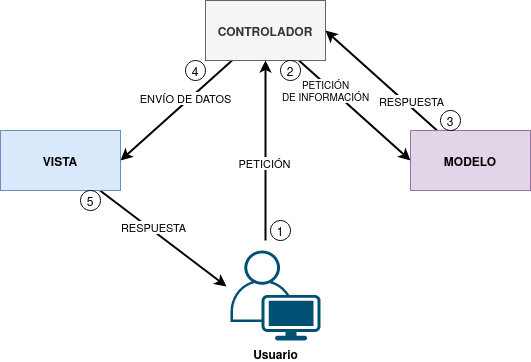
\includegraphics{../_static/images/mvc.png}
\caption{Diagrama que muestra la relación entre Modelo, Vista y
Controlador}\label{mvc}
}
\end{figure}

\begin{itemize}
\tightlist
\item
  \textbf{Modelo}: modifica, gestiona y actualiza los datos de la
  aplicación. En el caso de contar con una única base de datos, sería la
  capa donde se encuentra el código relacionado con las consultas,
  búsquedas, filtros y actualizaciones.
\item
  \textbf{Vista}: muestra al usuario final la interfaz gráfica de la
  aplicación, es decir, las páginas, ventanas, formularios, etc. En
  términos de programación se correspondería con el \emph{frontend}.
\item
  \textbf{Controlador}: gestiona, atiende y procesa las peticiones
  realizadas por parte de los usuarios. A través de esta capa se
  comunican el modelo y la vista. Como vemos en la \texttt{mvc}, el
  controlador solicita los datos necesarios al modelo, se manipulan
  acorde a la petición del usuario y se entregan a la vista de forma que
  el usuario pueda visualizar los resultados esperados.
\end{itemize}

\hypertarget{entorno-de-desarrollo-integrado-ide}{%
\section{Entorno de desarrollo integrado
(IDE)}\label{entorno-de-desarrollo-integrado-ide}}

\hypertarget{php-css-javascript-xml}{%
\subsection{\texorpdfstring{\emph{PHP} \textbar{} \emph{CSS} \textbar{}
\emph{JavaScript} \textbar{}
\emph{XML}}{PHP \textbar{} CSS \textbar{} JavaScript \textbar{} XML}}\label{php-css-javascript-xml}}

\begin{itemize}
\tightlist
\item
  Herramientas consideradas: \href{https://netbeans.org/}{NetBeans},
  \href{https://atom.io/}{Atom}, \href{https://eclipse.org/}{Eclipse},
  \href{https://www.zend.com/products/zend-studio}{Zend Studio} y
  \href{https://www.activestate.com/products/komodo-ide/}{Komodo}.
\item
  Herramienta elegida: \href{https://netbeans.org/}{NetBeans}.
\end{itemize}

NetBeans es un entorno de desarrollo muy completo escrito en Java.
Contiene una gran cantidad de funcionalidades y da soporte a todos y
cada uno de los lenguajes de programación utilizados en el desarrollo de
la infraestructura \emph{software}. Además, se pueden instalar
complementos que permiten extender su compatibilidad con otros marcos de
trabajo como \emph{Zend Framework}.

\hypertarget{latex}{%
\subsection{LaTeX}\label{latex}}

\begin{itemize}
\tightlist
\item
  Herramientas consideradas:
  \href{https://www.texstudio.org/}{TeXstudio} y
  \href{http://www.xm1math.net/texmaker/}{Texmaker}.
\item
  Herramienta elegida:
  \href{http://www.xm1math.net/texmaker/}{Texmaker}.
\end{itemize}

\emph{Texmaker} es un editor libre y gratuito para LaTeX distribuido
bajo la licencia GPL. Incluye múltiples herramientas necesarias para
elaborar documentos tanto con LaTeX como BibText o Metapost. También
incorpora funciones adicionales como la corrección ortográfica, el
auto-completado y plegado de código o un visor de pdf compatible con
SyncTeX y con modo de visualización continua. Además, es
multi-plataforma, disponible tanto en UNIX como en MacOS y Windows.

\hypertarget{generador-de-documentaciuxf3n}{%
\section{Generador de
documentación}\label{generador-de-documentaciuxf3n}}

\begin{itemize}
\tightlist
\item
  Herramientas consideradas:
  \href{https://www.sphinx-doc.org/es/master/index.html}{Sphinx} y
  \href{https://www.mkdocs.org/}{Mkdocs}.
\item
  Herramienta elegida:
  \href{https://www.sphinx-doc.org/es/master/index.html}{Sphinx}.
\end{itemize}

He decidido utilizar el generador de documentación \emph{Sphinx} ya que
es mucho más completo que \emph{MkDocs}. Además de soportar el lenguaje
de marcado ligero \emph{Markdown} es compatible con
\emph{reStructuredText}. Esta compatibilidad hace que sea posible usar
ambos lenguajes en un mismo proyecto \emph{Sphinx}. Además, con el uso
del conversor \href{http://pandoc.org/}{Pandoc}, toda la documentación
generada a partir de ambos lenguajes se puede exportar a multitud de
formatos, entre los que se encuentra LaTeX.

\emph{Markdown} es un lenguaje muy conocido debido a que es utilizado en
plataformas como \emph{Github} o \emph{StackOverflow}. Fue creado para
generar contenido de una manera sencilla de escribir y fácil de leer.
Permite además convertir el texto marcado en documentos \emph{XHTML}.

\emph{reStructuredText} presenta también una sintaxis sencilla y de
fácil lectura. La principal ventaja respecto a \emph{Markdown} es que
permite elaborar expresiones más complejas sin el uso de
librerías/aplicaciones externas.

\emph{LaTeX} es el estándar de facto para la publicación de documentos
científicos. Permite la creación de documentos con una alta calidad
tipográfica. Utiliza \emph{Tex} como motor a la hora de darle formato a
los documentos.

\hypertarget{herramientas-de-integraciuxf3n-continua}{%
\section{Herramientas de integración
continua}\label{herramientas-de-integraciuxf3n-continua}}

\hypertarget{compilaciuxf3n-y-despliegue}{%
\subsection{Compilación y
Despliegue}\label{compilaciuxf3n-y-despliegue}}

\begin{itemize}
\tightlist
\item
  Herramientas consideradas:
  \href{https://github.com/features/actions}{Github Actions},
  \href{https://travis-ci.org/}{Travis CI} y
  \href{https://jenkins.io/}{Jenkins}.
\item
  Herramienta elegida: \href{https://github.com/features/actions}{Github
  Actions}.
\end{itemize}

Para aplicar la integración continua al proyecto se ha dedicido utilizar
\emph{Github Actions}. El principal motivo de esta elección es que todas
sus funciones se encuentran integradas en la propia interfaz de
\emph{Github}, lo que facilita en gran medida su uso. Además, permite
reutilizar código elaborado por otros usuarios de la comunidad en los
flujos de trabajo (\emph{workflows}) personales.

\hypertarget{calidad-del-cuxf3digo}{%
\subsection{Calidad del código}\label{calidad-del-cuxf3digo}}

\begin{itemize}
\tightlist
\item
  Herramientas consideradas: \href{https://codacy.com}{Codacy},
  \href{https://codecov.io/}{Codecov} y
  \href{https://codeclimate.com/}{CodeClimate}.
\item
  Herramienta elegida: \href{https://codacy.com}{Codacy}.
\end{itemize}

La opción escogida ha sido \emph{Codacy} ya que, de entre las tres
propuestas, es la que está más enfocada a la revisión de código
automatizada, que es lo se estaba buscando. Da soporte a todos los
lenguajes que se han utilizado en el proyecto ( \emph{PHP}, \emph{HTML},
\emph{JavaScript} y \emph{CSS} ). Además, el proceso de configuración no
se hace nada pesado gracias a que se puede llevar a cabo desde su propia
interfaz gráfica. Entre sus configuraciones más utilizadas están la
exclusión de ficheros, la activación/desactivación de patrones de
código, la selección de ramas y la gestión de integraciones.

\hypertarget{documentaciuxf3n-continua}{%
\subsection{Documentación continua}\label{documentaciuxf3n-continua}}

\href{https://readthedocs.org/}{Read the Docs} es una plataforma web que
facilita la tarea de documentar productos \emph{software} automatizando
la compilación, versionado y hospedaje de los ficheros generados por la
herramienta de documentación \emph{Sphinx}. El proceso es muy sencillo,
basta con alojar la documentación \emph{Sphinx} en un repositorio,
realizar un \emph{commit} sobre este y, automáticamente, se actualizan
los cambios en la documentación alojada en \emph{readthedocs.org}.
Presenta múltiples formatos de exportación y permite configurar
múltiples aspectos (traducciones, variables de entorno, reglas de
automatización, etc.). Todos estos servicios se ofrecen de forma
gratuita.

\hypertarget{herramienta-de-diagramaciuxf3n}{%
\section{Herramienta de
diagramación}\label{herramienta-de-diagramaciuxf3n}}

\begin{itemize}
\tightlist
\item
  Herramientas consideradas:
  \href{https://es.libreoffice.org/descubre/draw/}{Draw - LIbreOffice},
  \href{https://www.smartdraw.com/}{SmartDraw} y
  \href{https://app.diagrams.net/}{Draw.io}.
\item
  Herramienta elegida: \href{https://app.diagrams.net/}{Draw.io}.
\end{itemize}

\emph{Draw.io} es una herramienta gratuita de diseño que permite crear y
compartir diagramas \emph{on-line}, es decir, sin necesidad de instalar
programa alguno. Presenta una interfaz elegante y fácil de utilizar
desde la cual podemos hacer uso de sus múltiples funciones como, por
ejemplo, importar imágenes, añadir objetos UML, exportar e importar
proyectos en diversos formatos, etc.

\hypertarget{herramientas-de-comunicaciuxf3n}{%
\section{Herramientas de
comunicación}\label{herramientas-de-comunicaciuxf3n}}

\hypertarget{microsoft-teams}{%
\subsection{\texorpdfstring{\emph{Microsoft
Teams}}{Microsoft Teams}}\label{microsoft-teams}}

A través de
\href{https://www.microsoft.com/es-es/education/products/teams}{Microsoft
Teams} se han llevado a cado las reuniones de cada \emph{sprint}.
\emph{Teams} viene integrado en el paquete de \emph{Microsoft Office
365}, por lo que es un servicio que puede ser adquirido por el personal
de la UBU. Ofrece una gran cantidad de funcionalidades relacionadas con
la comunicación como, por ejemplo, la creación de chats personalizados
(individuales/grupales, públicos/privados, etc.), compartición de
pantalla, integración de aplicaciones externas (Stream, Excel, etc.) o
introducción de efectos de cámara (efectos de fondo, filtros, etc.).

\hypertarget{zoom}{%
\subsection{\texorpdfstring{\emph{Zoom}}{Zoom}}\label{zoom}}

{Zoom \textless https://zoom.us/\textgreater{}} es la herramienta de
comunicación con la que se han llevado a cabo las reuniones tanto con el
CENIEH como con ARIADNEplus. Al igual que la herramienta \emph{Microsoft
Teams}, permite realizar videollamadas y reuniones virtuales con
multitud de funcionalidades extra.

\hypertarget{otras-herramientas}{%
\section{Otras herramientas}\label{otras-herramientas}}

\hypertarget{docker}{%
\subsection{\texorpdfstring{\emph{Docker}}{Docker}}\label{docker}}

La tecnología \href{https://www.docker.com/}{Docker} permite desplegar
una aplicación distribuida y empaquetarla junto a todas sus dependencias
y librerías en un uno o varios "objetos" denominados contenedores o
\emph{containers}. Estos pueden ser ejecutados en cualquier servidor
Linux, aumentando así la flexibilidad y portabilidad de nuestra
aplicación.

\hypertarget{google-cloud}{%
\subsection{\texorpdfstring{\emph{Google
Cloud}}{Google Cloud}}\label{google-cloud}}

\href{https://cloud.google.com/}{Google Cloud} es una plataforma creada
por la compañía \emph{Google} desde la que puedes acceder a numerosos
servicios relacionados con el desarrollo web. Alguno de sus servicios
son: \emph{Cloud Computing}, \emph{Networking}, \emph{Data Storage},
\emph{Data Analytics}, \emph{Machine learning}, etc.

\hypertarget{gke-google-kubernetes-engine}{%
\subsubsection{\texorpdfstring{\emph{GKE -- Google Kubernetes
Engine}}{GKE -- Google Kubernetes Engine}}\label{gke-google-kubernetes-engine}}

\href{https://cloud.google.com/kubernetes-engine}{Google Kubernetes
Engine} (GKE) proporciona un entorno desde donde puedes implementar,
administrar y escalar aplicaciones en contenedores mediante la
infraestructura de \emph{Google}. El entorno de GKE consta de varias
máquinas (en particular, instancias de \emph{Compute Engine}) que se
agrupan para formar un clúster.

\hypertarget{kubernetes}{%
\subsection{\texorpdfstring{\emph{Kubernetes}}{Kubernetes}}\label{kubernetes}}

\href{https://kubernetes.io/es/}{Kubernetes} es una plataforma
\emph{open-source} que permite automatizar los procesos relacionados con
la implementación, administración y escalabilidad de contenedores. He
decidido utilizar este orquestador (\emph{orchestrator}) para desplegar
mi aplicación en la nube (\emph{Google Cloud}) por la gran cantidad de
ventajas que ofrece como, por ejemplo, autoreparación de contenedores,
utilización de \emph{secrets} o despliegues y rollbacks automáticos.

\hypertarget{kustomize}{%
\subsection{\texorpdfstring{\emph{Kustomize}}{Kustomize}}\label{kustomize}}

\href{https://github.com/kubernetes-sigs/kustomize}{Kustomize} es una
herramienta que permite operar sobre objetos de la plataforma
\emph{Kubernetes} a través de un archivo de personalización.

\end{document}

\capitulo{5}{Aspectos relevantes del desarrollo del proyecto}

A continuación se van a mostrar los aspectos más relevantes del
desarrollo del proyecto, justificando las decisiones tomadas y dando
visibilidad a los problemas encontrados.

\section{Ciclo de vida del proyecto}

El 01 de febrero de 2020, se inició este proyecto con el objetivo de
llevar a cabo el proceso de integración de los datos del \emph{CENIEH} en
\emph{ARIADNEplus}. Adicionalmente, se propuso implantar en el\emph{CENIEH} una
infraestructura \emph{software} mediante la cual sus investigadores
fueran capaces de llevar a cabo las tareas de integración por sí
solos. De esta manera, a través de la infraestructura propuesta, serían
capaces de continuar con las labores de integración una vez concluido el
periodo de colaboración entre el \emph{CENIEH} y la \emph{UBU}.

El proyecto tiene una duración total de 6 meses, lo que significa
que el 01 de agosto de 2020 dará por concluido el periodo de colaboración entre
el CENIEH y la UBU. 

Las fases en las que se puede dividir el proyecto son:

\begin{itemize}
\tightlist
\item
  \textbf{Investigación}: en esta fase se realiza un estudio previo del
  proyecto ARIADNEplus, así como de los conjuntos de datos del CENIEH
  que están involucrados en el proceso de integración.
\item
  \textbf{Desarrollo}: a lo largo de esta fase se ejecutan todas las
  tareas relacionadas con el diseño, desarrollo e implementación de la
  infraestructura \emph{software}.
\item
  \textbf{Integración}: en esta fase se integran los datos del CENIEH en
  ARIADNEplus haciendo uso tanto de la infraestructura \emph{software}
  implementada como de los servicios ofrecidos por ARIADNEplus.
\end{itemize}


\section{Investigación}

Durante las primeras semanas de trabajo, se llevó a cabo un estudio
exhaustivo del proyecto \emph{ARIADNEplus}, especialmente del \textbf{proceso
de integración} al que cada miembro debía someter sus datos. A medida
que se iban aprendiendo nuevos aspectos, se comprobaba su compatibilidad
con los datos propuestos por el \emph{CENIEH}, anotando en todo momento los
problemas que pudieran surgir.


\subsection{Proceso de integración}

emph{ARIADNEplus} no agrega ni mueve datos de los sistemas de información de
los miembros del proyecto, solo añade \textbf{metadatos} a los conjuntos
de datos que son mantenidos y gestionados por cada miembro. Este tipo de 
información debe adoptar un \textbf{esquema o modelo} para poder ser
representado a través de catálogos o repositorios. En el caso de
emph{ARIADNEplus}, cuentan con un esquema denominado \textbf{AO-Cat}
(\textbf{A}RIADNE \textbf{O}ntology \textbf{-} \textbf{Cat}alog),
diseñado exclusivamente para el proyecto.

Cada miembro del proyecto, incluído el \emph{CENIEH}, cuenta desde un principio
con sus propias colecciones de metadatos. Esto puede considerarse un
problema ya que, como se ha comentado anteriormente, este tipo de
información se representa a través de un esquema, el cual será distinto
en cada uno de los miembros. Ante esta situación, al no coincidir el
esquema de origen (?) con el de destino (AO-Cat), sería imposible poder
representar los datos del origen en el catálogo.

\imagen{mappingProblem}{Conflicto entre esquemas de metadatos distintos}{0.9}

Además, un esquema está formado por un conjunto de elementos, cada uno
de los cuales está sujeto a unas determinadas \textbf{reglas}. Por ejemplo,
podría especificarse el tipo de dato que almacena (\emph{string},
\emph{date}, etc.) o considerarse como imprescindible (no nulo). Este
hecho aumenta aún más la complejidad del proceso de integración ya que
cada miembro cuenta con sus propios elementos y con sus propias reglas.

Para dar solución a todos estos problemas, \emph{ARIADNEplus} propone dividir
el proceso de integración en 6 fases.

\imagen{integrationPhases}{Representación gráfica de las fases en las que se divide el proceso de integración}{0.9}

\begin{enumerate}
\def\labelenumi{\arabic{enumi}.}
\tightlist
\item
  \textbf{Confirmación}: se confirman las colecciones de metadatos que
  serán agregadas y, además, se indica a qué categoria de datos de
  \emph{ARIADNEplus} pertenecen.
\item
  \textbf{Transformación}: una vez estén listos los metadatos de origen,
  se genera un fichero de definición de mapeo que permita transformar el
  esquema de metadatos de origen al esquema objetivo (\emph{AO-Cat}).
\item
  \textbf{Enriquecimiento}: se mejora la calidad de los metadatos
  sometiendo los datos a un proceso de enriquecimiento utilizando el
  vocabulario \emph{Getty AAT} y/o \emph{PeriodO}.
\item
  \textbf{Importación}: habiendo completado las tres fases anteriores,
  se ejecuta el proceso de importación de los metadatos.
\item
  \textbf{Simulación de publicación}: con los metadatos de origen ya
  importados en la base de datos, se realiza una simulación de
  publicación.
\item
  \textbf{Publicación}: si los resultados obtenidos en la fase 5 son
  favorables, se lleva a cabo la publicación de los metadatos en el
  catálogo oficial.
\end{enumerate}

\subsubsection{Confirmación}

En esta fase se confirman qué colecciones de datos serán integradas en
el proyecto. Además, se debe indicar a qué categoría de datos de \emph{ARIADNE}
pertenecen.

\imagen{categoriesARIADNE}{Fase de confirmación.}{0.9}

Afortunadamente, los datos propuestos por el \emph{CENIEH} se obtuvieron con suma facilidad,
sin ningún tipo de reticencia por su parte. 

En la siguiente tabla se indican las principales características de cada una de las
colecciones de datos confirmadas para la integración con \emph{ARIADNEplus}.
Además, se especifica la categoría \emph{ARIADNE} a la que corresponden.

\begin{table}[H]\label{tabla:datos}
\centering
\resizebox{\textwidth}{!}{\begin{tabular}{@{}llllll@{}}
\hline
Colección          & Núm. Registros & Docs asociados & Campos                                                                                                                                                                                                                                                                                           & Formato & Categoría ARIADNE   \\ \hline
Anatomía Comparada & 571            & Sí             & \begin{tabular}[c]{@{}l@{}}SIGNA\_CENIEH, Clase, Orden,\\ Familia Género, Especie,\\ Sigla de campo, Elemento,\\ Sexo, Adulto Localidad,\\ Municipio, Provincia, Pais,\\ Tipo de objeto\end{tabular}                                                                                             & CSV     & Scientific analysis \\ \hline
Litoteca           & 99             & Sí             & \begin{tabular}[c]{@{}l@{}}Afloramiento, Sigla,\\ Localización, Datum, X, Y, Z,\\ Acceso, Tipo de Afloramiento,\\ Tipo de roca, Depositante,\\ Muestra física, Lámina\\ delgada, Laboratorio geología\\ CENIEH, Fotografías, Otros\\ datos, Topografía\end{tabular}                              & CSV     & Scientific analysis \\ \hline
Ratón Pérez        & 1323           & Sí             & \begin{tabular}[c]{@{}l@{}}Sigla, Individuo, Sexo, Edad,\\ Pieza, Superior/inferior,\\ Lado, Conservación,\\ Consolidado, Pegado,\\ Observaciones, Localización,\\ Fecha MicroCT, Archivo mCT,\\ Proyecto Amira, localización,\\ No Imágenes, kv/mA, Vxl,\\ Size, Filter, Fotos mCT\end{tabular} & CSV     & Scientific analysis \\ \hline
Sedimentos         & 7695           & No             & \begin{tabular}[c]{@{}l@{}}ReferenciaBolsa,\\ ReferenciaCaja, Yacimiento,\\ Nivel, Cuadro, Z, Situacion,\\ FechaRecogida, FechaAlmacen,\\ FechaProcesando\end{tabular}                                                                                                                           & CSV     & Scientific analysis \\ \hline
CIR                & 1853           & Sí             & Dublin Core terms                                                                                                                                                                                                                                                                              & CSV     & Scientific analysis \& Fieldwork Reports \\ \hline
\end{tabular}}\\
\caption{Colecciones de metadatos propuestas por el \emph{CENIEH} para la
integración con \emph{ARIADNEplus}.}
\end{table}

\subsubsection{Transformación}

Para evitar el problema mostrado en la \texttt{mappingProblem},
ARIADNEplus pone a disposición de sus miembros la \textbf{herramienta
\emph{X3ML Mapping Tool}}, disponible en el entorno virtual \emph{ARIADNEplus Mappings} del
portal \emph{ARIADNEplus Gateway} de \emph{D4Science}. Está compuesta
por un conjunto de microservicios, de código abierto, que siguen el
modelo de referencia \emph{SYNERGY} \cite{art:syn} para la transmisión y agregación de
datos.

\imagen{transformARIADNE}{Fase de transformación.}{0.9}

Los componentes clave de este servicio son:

\begin{itemize}
\tightlist
\item
  \emph{\textbf{3M -- Mapping Memory Manager}}: herramienta utilizada para la
  gestión de archivos de definición de mapeo. Proporciona una serie de
  acciones administrativas que ayudan a los proveedores de datos a
  administrar sus archivos de definición de mapeo.
\end{itemize}

\imagen{mmm3m}{Vista de la herramienta \emph{Mapping Memory Manager - 3M}}{0.9}

\begin{itemize}
\tightlist
\item
  \emph{\textbf{3M Editor}} provee la interfaz que permite crear asignaciones
  entre los elementos del esquema de metadatos a mapear y el esquema
  objetivo.
\end{itemize}

\imagen{3meditor}{Vista de la herramienta \emph{3M Editor}}{0.9}

\begin{itemize}
\tightlist
\item
  \emph{\textbf{X3ML Engine}}: ejecuta la transformación de los elementos de
  origen al formato de destino. Tomando como entrada los datos de origen
  (en formato XML), la descripción de las asignaciones existentes en el
  fichero de definición de mapeo y el archivo que contiene las políticas
  para la generación de URIs, es responsable de transformar el documento
  original en un documento RDF válido que corresponda al archivo XML de
  entrada con las asignaciones y políticas indicadas.
\item
  \emph{\textbf{RDF visualizer}}: permite, de una forma rápida, inspeccionar los
  documentos transformados.
\end{itemize}

\imagen{rdfvisualizer}{Vista de la herramienta \emph{RDF visualizer}.}{0.6}

Esta herramienta toma un \textbf{papel decisivo} en el proceso de
integración ya que permite transformar el modelo de origen al esquema de
metadatos utilizado en \emph{ARIADNEplus} (\emph{AO-CAT}).

A continuación se van a describir los \textbf{principales \textbf{retos}} a los
que nos hemos tenido que enfrentar durante esta segunda fase:

\begin{itemize}
\tightlist
\item
  Todos los conjuntos de datos propuestos por el CENIEH están en formato
  CSV. Esto supone un problema ya que \textbf{ARIADNEplus solo trabaja
  con ficheros XML}, es decir, no cuenta con ningún método de
  importación que tolere archivos CSV.
\item
  \textbf{Los conjuntos de datos del CENIEH}, a excepción de la
  colección del CIR, están dispuestos de forma irregular, es decir,
  \textbf{no siguen ningún esquema estandarizado}. Esto implica que para
  cada conjunto de datos, se necesita hacer un fichero de definición de
  mapeo distinto, lo que no es para nada eficiente.
\item
  En el esquema objetivo, los \textbf{elementos} pueden ser opcionales u
  \textbf{obligatorios}. Los elementos opcionales no suponen ningún
  problema ya que pueden quedar vacíos, sin embargo, los elementos
  obligatorios requieren la existencia de un elemento en el modelo de
  origen que pueda sustituirlo, es decir, que tenga el mismo
  significado. Esta regla supone un reto para el CENIEH ya que muchos de
  los elementos obligatorios no cuentan con un elemento apto en las
  colecciones de datos propuestas.
\item
  \textbf{El contenido} almacenado en cada elemento del esquema objetivo
  \textbf{ha de tener un formato específico}. Por ejemplo, el contenido
  del elemento \emph{has\_language}, responsable de indicar el idioma en
  el que está dispuesto el objeto al que referencia, debe cumplir con el
  estándar ISO639-1 o ISO639-2. Por tanto, el elemento asignado en el
  origen debe seguir el mismo formato.
\end{itemize}


\subsubsection{Enriquecimiento}

En ocasiones, los metadatos por si solos no son lo suficientemente
precisos o claros como para describir una determinada característica del
objeto al que se refieren. En el caso de la arqueología, existen
multitud de conceptos con un alto grado de complejidad que necesitan ser
explicados en detalle. Por este motivo, \emph{ARIADNEplus} propone enriquecer
los metadatos haciendo uso del vocabulario \emph{Getty AAT} y del
cliente \emph{PeriodO}.

\imagen{enrichment}{Enriquecimiento de metadatos}{0.9}

En la Figura \ref{fig:enrichment} se muestra el flujo de datos del proceso de
enriquecimiento de metadatos. Por una parte, vemos un archivo .json, el
cual se obtiene a través de la \textbf{herramienta \emph{Vocabulary Matching
Tool}}. Esta es otra de las herramientas que se pueden encontrar en el
entorno virtual \emph{ARIADNEplus Mappings}. Permite mapear el vocabulario utilizado
en el documento de origen al vocabulario \emph{Getty AAT}.

\imagen{vmt}{Vista de la herramienta \emph{Vocabulary Matching Tool}}{0.9}

El archivo generado por esta herramienta (.json) define las relaciones
entre los términos del vocabulario de origen y los términos del
vocabulario \emph{Getty AAT}. Desde el catálogo de \emph{ARIADNEplus}, todos
aquellos términos que tengan una asociación definida, serán hiperenlaces
que apunten al término \emph{Getty AAT} asociado.

Además, vemos representada la base de datos donde \textbf{PeriodO} almacena sus
registros. Para aportar información adicional a los periodos existentes
en nuestros datos, debemos publicar en el cliente de \emph{PeriodO} nuestra
propia colección de periodos. De esta forma, \emph{ARIADNEplus} podrá recoger
desde la BD de \emph{periodO} nuestra colección para, posteriormente,
establecer una relación entre los periodos de un lado y de otro. Al
igual que con el vocabulario, todos los periodos que tengan una
asociación definida, serán hiperenlaces que apunten al objeto de
\emph{periodO}.

En esta fase se encontraron varios \textbf{inconvenientes}: 

\begin{itemize}
\tightlist
\item
  Muchos de los términos existentes en los conjuntos de datos del CENIEH no están
  presentes en el vocabulario \emph{Getty AAT}. Por este motivo, solo se
  pudo enriquecer una pequeña parte del conjunto total.
\item
  Para poder publicar la colección en \emph{periodO}, se requería determinar la autoridad de
  los periodos, es decir, indicar de donde procedían. Desde el CENIEH no
  me pudieron facilitar ese dato ya que lo desconocían. Por este motivo,
  no se pudo llevar a cabo la publicación y por ende no se enriquecerieron
  los periodos.
\end{itemize}

\subsubsection{Importación}

El sistema de importación de \emph{ARIADNEplus}, conocido como \emph{ARIADNEplus}
\emph{Aggregator}, se basa en el kit de herramientas de \emph{software}
D-Net (implementado y mantenido por \emph{ISTI-CNR} \cite{weboff:isti}), 
que proporciona funciones integradas que permiten recopilar conjuntos 
de metadatos a través de múltiples métodos. Está disponible en el portal 
\emph{ARIADNEplus Gateway}, sin embargo, su acceso está restringido a los 
coordinadores del proyecto. 

Las principales opciones de importación son:

\begin{enumerate}
\def\labelenumi{\arabic{enumi}.}
\tightlist
\item
  \textbf{OAI-PMH} \cite{weboff:oai}: es un protocolo estándar para el intercambio de
  metadatos. A través de este método \emph{ARIADNEplus} puede recolectar los
  metadatos almacenados en un repositorio de forma remota.
\item
  \textbf{SFTP} \cite{weboff:sftp} : es un protocolo de transmisión de ficheros. Esta opción
  es algo engorrosa ya que debe existir un archivo XML por recurso, es
  decir, no puedes agrupar varios registros en un mismo fichero XML. Los
  socios son responsables del servidor SFTP. Se admiten modos de
  autentificación.
\item
  \textbf{FTP(S)} \cite{weboff:ftp}: es otro protocolo de transferencia de ficheros.
  Presenta las mismas características de importación que SFTP.
\item
  \textbf{Workspace}: se pueden subir directamente los registros en el
  \emph{workspace} de \emph{D4Sciente} (\emph{ARIADNEplus Gateway}). Cada socio tiene
  su propia carpeta donde puede ir almacenando los documentos \emph{XML}
  (metadatos) que desee importar.
\end{enumerate}

Dado que este sistema es inaccesible para la mayoría de los miembros
(incluido el \emph{CENIEH}), se debe escoger una de esas opciones y
comunicársela al coordinador responsable. Una vez realizada la
importación, se deben facilitar tres datos:

\begin{enumerate}
\tightlist
\item
  Qué ficheros (\emph{.xml}) de los importados se desean publicar.
\item
  Cuál es el identificador del fichero de definición de mapeo (e.g.
  \emph{Mapping/621}) que transformará el esquema de metadatos presente
  en tus ficheros al esquema \emph{AO-Cat}.
\item
  Opcionalmente, el enlace a tu colección de \emph{periodO} y/o el fichero de
  mapeo (\emph{.json}) del vocabulario.
\end{enumerate}

Los conjuntos de datos del \emph{CENIEH} están almacenados de forma local,
exceptuando el \emph{CIR}. Por ello, de entre todas las opciones posibles, la
única forma válida de importar metadatos sería a través del
\emph{Workspace}.

\subsubsection{Simulación de publicación}

Una vez establecida la comunicación con el coordinador responsable del
proceso de importación, se debe esperar a su respuesta. Dependiendo del
contenido de esta, se pueden tomar dos caminos:

\begin{enumerate}
\def\labelenumi{\arabic{enumi}.}
\tightlist
\item
  Nos indican que todas las partes del proceso (metadatos, mapeo,
  enriquecimiento) son correctos. En tal caso, los metadatos propuestos
  estarían ya disponibles desde el portal fantasma de \emph{ARIADNEplus}. Este
  es idéntico al original con la única diferencia de que sólo tienen
  acceso los miembros del proyecto.
\item
  Nos indican que alguna parte del proceso no es correcta. Ante esta
  situación, se debe volver hacia atrás en el proceso de integración
  para solventar los conflictos señalados por el coordinador.
\end{enumerate}

\subsubsection{Publicación}

Si en la fase previa se ha obtenido una respuesta satisfactoria, el
miembro que inició el proceso de integración sería ya capaz de observar
el resultado final sobre el portal fantasma. 

Una vez visualizado el resultado, deberá comunicarse de nuevo con el
responsable de la importación para indicarle sus impresiones. Se pueden
dar dos situaciones:

\begin{enumerate}
\def\labelenumi{\arabic{enumi}.}
\tightlist
\item
  El resultado es favorable. Ante esta situación el coordinador lleva a
  cabo la publicación de los datos en el portal real.
\item
  No se esperaba el resultado obtenido. En tal caso, se deben mantener
  las conversaciones hasta llegar a una solución.
\end{enumerate}

En el caso de que todo haya salido según lo planeado, el proceso de
integración para los conjuntos de datos publicados quedaría suspendido.
Existe la posibilidad de reactivar este proceso en el caso de que se
deseen actualizar o añadir datos, sin embargo, hay que tener en cuenta
que cualquier cambio en la estructura de los datos supondría tener que
volver a realizar el proceso desde cero.

\section{Desarrollo}

Recordemos que en la fase anterior se anotaron todos los aspectos
relevantes del proceso de integración, incluyendo además los problemas
de incompatibilidad encontrados entre dicho proceso y los datos
propuestos por el CENIEH. 

Es en esta fase cuando se aplican las competencias y los conocimientos 
adquiridos a lo largo del grado con el objetivo de desarrollar una infraestructura 
\emph{software} que sea capaz de guiar a los operarios del CENIEH en el proceso de integración
y, además, resuelva los problemas mencionados en la fase anterior.

\subsection{\emph{Omeka} como aplicación principal}

Desarrollar desde cero una infraestructura \emph{software} que cumpliera
con todos los requisitos propuestos no era viable debido a la limitación
temporal del proyecto. Por este motivo, se decidió utilizar
\emph{software} de terceros que cumpliera con un mínimo de
\textbf{requisitos}:

\begin{itemize}
\tightlist
\item
  Permitir la \textbf{gestión de metadatos}: los archivos de información
  involucrados son metadatos, por tanto, se necesita un sistema que
  permita realizar todo tipo de tareas de gestión sobre este tipo de
  datos.
\item
  Disponer de \textbf{herramientas de importación y exportación}: los
  datos de origen necesitarán ser importados a la plataforma para
  realizar sobre ellos las operaciones oportunas. Una vez gestionados,
  deberán ser exportados para someterlos al proceso de integración.
\item
  Ser \textbf{software libre}: este requisito era fundamental ya que,
  para poder adaptar la infraestructura a las necesidades del proyecto,
  se debe tener total libertad a la hora de ejecutar, copiar,
  distribuir, estudiar, modificar y mejorar el \emph{software}.
\end{itemize}

Se consideraron varios productos \emph{software} para acabar escogiendo
\href{https://omeka.org/classic/}{Omeka Classic}. Una de las
características que hacen de la aplicación una magnífica plataforma para
el proyecto es su \textbf{escalabilidad}. Gracias a su sistema de
\textbf{complementos} o \emph{plugins}, cualquier programador tiene la
posibilidad de adaptarla a sus necesidades individuales sin tener que
modificar el código base de la aplicación.

Actualmente, \emph{Omeka} cuenta con una gran cantidad de \emph{plugins}
disponibles tanto en su \href{https://omeka.org/classic/plugins/}{página
oficial} como en
\href{https://daniel-km.github.io/UpgradeToOmekaS/omeka_plugins.html}{Github}.
Esto es posible gracias a la extensa comunidad de usuarios que le
respalda. 

Parte de los \emph{plugins} publicados se han podido utilizar para
adaptar la infraestructura a las necesidades del proyecto, sin embargo,
se han tenido que desarrollar nuevos \emph{plugins} para cubrir
requisitos específicos. Además, se han llevado a cabo modificaciones
sobre alguno de los \emph{plugins} de terceros utilizados.

Por este motivo, la mayoría de las tareas realizadas en esta fase están directamente
relacionadas con la creación y modificación de \emph{plugins} para \emph{Omeka}.

\subsubsection{Complementos o \emph{plugins}}

Los complementos o \emph{plugins} son capaces de añadir nuevas
funcionalidades a \emph{Omeka} gracias a que esta tiene implementado un
sistema de ganchos o \emph{hooks}. Estos nos permiten acoplar código en
puntos específicos del flujo de ejecución de la aplicación, evitando así
tener que alterar el código base de esta.

Dentro de la aplicación se pueden encontrar dos tipos distintos de
\emph{hooks}: \textbf{\emph{hooks} de acción} y \textbf{filtros (\emph{filters})}.


\paragraph{\emph{Hooks} de acción.}

Este tipo de \emph{hook} permite añadir la ejecución de funciones externas en
puntos de ejecución específicos.

Por ejemplo, en el caso de que se quiera introducir un formulario en una
página de \emph{Omeka}, se debería utilizar el \emph{hook}
alojado en dicha página para ejecutar la función encargada de imprimir
el código HTML del formulario. En este ejemplo, la función no retornaría
nada ya que se limita a imprimir código, y es que en este tipo de
\emph{hooks} la función no tiene por qué devolver nada.

En los archivos de \emph{Omeka} se pueden localizar estos \emph{hooks} buscando
la función \emph{fire\_plugin\_hook()}. Una vez encontrada, desde el
\emph{plugin} que estamos desarrollando, haciendo uso de la interfaz
\emph{Omeka\_Plugin\_AbstractPlugin}, bastaría con añadir este
\emph{hook} a la lista \emph{\_hooks} e instanciar el método
correspondiente, el cual siempre tiene la nomenclatura
\emph{hook\textless NombreDelHook\textgreater()}.

\imagen{actionhooks}{Ejemplo de \emph{action hook}.}{1}

En el ejemplo vemos como \emph{fire\_plugin\_hook()} tiene dos
parámetros de entrada, el primero indica el nombre del \emph{hook} y el
segundo almacena los argumentos de entrada que tendrá la función que
almacena la acción.


\paragraph{Filtros (\emph{Filters}).}

Los filtros permiten, al igual que los \emph{hooks} de acción, ejecutar
funciones externas en puntos específicos de la aplicación. Sin embargo,
el objetivo de estos es algo distinto ya que no pretenden modificar
código sino alterar los datos de una determinada variable.

Las funciones deben tener un parámetro de entrada y otro de
salida de forma que, desde el interior de la función, se procesa el
valor de entrada y se devuelve el valor resultante.

En los archivos de \emph{Omeka} se pueden localizar estos \emph{filters}
buscando la función \emph{apply\_filters()}. Una vez encontrada, existen
dos formas de usar ese filtro:

\begin{enumerate}
\def\labelenumi{\arabic{enumi}.}
\tightlist
\item
  Utilizando la interfaz \emph{Omeka\_hooksPlugin\_AbstractPlugin} es posible
  utilizar el filtro añadiendo su nombre a la lista \emph{\_filters}. A
  continuación, se añadiría el método público con el nombre
  \emph{filter} seguido del nombre del filtro.
\end{enumerate}

\imagen{filterhooksA}{Ejemplo de \emph{filter hook}.}{1}

\begin{enumerate}
\def\labelenumi{\arabic{enumi}.}
\setcounter{enumi}{1}
\tightlist
\item
  Utilizando el método \emph{add\_filter()}, se puede utilizar el filtro
  pasando como primer parámetro el nombre del filtro implicado y como
  segundo parámetro la función que se ejecutará. En este caso, el nombre
  de la función es personalizable. Además, se puede pasar un tercer
  parámetro para indicar la prioridad de nuestro \emph{hook}, es decir,
  si existiera más de un \emph{plugin} utilizando ese mismo filtro, se
  ejecutaría la función de cada uno en función de su prioridad, de mayor
  a menor prioridad. Por defecto, todos los \emph{filtros} de cada
  \emph{plugin} tienen una prioridad de 10, por lo que el orden de
  ejecución se determina por la fecha de instalación, de más antiguos a
  más nuevos.
\end{enumerate}

\imagen{filterhooksB}{Segundo ejemplo de \emph{filter hook}.}{0.9}

\subsection{Entornos de trabajo}

Durante la fase de desarrollo, se ha trabajado sobre dos entornos:

\begin{itemize}
\tightlist
\item
  \textbf{Entorno de desarrollo}: se actualiza al cometer cambios sobre
  la rama \emph{develop}. Permite llevar un seguimiento diario del
  estado de la aplicación durante el desarrollo de la misma. Es público.
\item
  \textbf{Entorno de producción}: se actualiza al cometer cambios sobre
  la rama \emph{main}. En su interior se puede encontrar una versión
  estable de la aplicación. El intervalo de tiempo de actualización gira
  entorno a las dos semanas. Es privado, sólo tienen acceso los miembros
  del \emph{CENIEH}.
\end{itemize}


\subsection{Despliegue de la infraestructura}

Para llevar a cabo el despliegue de la infraestructura se ha utilizado
la herramienta \emph{Github Actions}. Dependiendo del entorno de
trabajo, se ha procedido de una manera u otra:


\subsubsection{Servidor de desarrollo}

A través de la herramienta \emph{Github Actions} se ha automatizado el
despliegue de la infraestructura sobre el servidor de desarrollo. A esta
técnica se la conoce como despliegue continuo.

\imagen{cicd}{Despliegue continuo de la aplicación.}{0.9}

En la \texttt{cicd} he representado el proceso mediante el cual se lleva
a cabo el despliegue. Con el \emph{workflow} configurado y alojado en la
ruta \emph{.github/workflows} de mi repositorio en GitHub, cuando
ejecuto un \emph{push} sobre la rama \emph{develop}, si los cambios
cometidos afectan a cualquier carpeta que no sea la de \emph{/docs}, se
ejecutan las acciones correspondientes al despliegue de mi aplicación,
las cuales se pueden apreciar en la imagen.


\subsubsection{Servidor de producción}

Sobre el servidor de producción no se ha podido automatizar el
despliegue debido a que el acceso a este era privado, es decir, no se
podía establecer comunicación desde el exterior sin previa conexión al
VPN del CENIEH y el posterior acceso vía \emph{ssh} al servidor.

\imagen{dockerdeploy}{Despliegue "semi-continuo" de la aplicación.}{0.9}

Como solución a este inconveniente, se automatizó por separado la
compilación y publicación de la imagen \emph{Docker} asociada a nuestra
aplicación. De esta manera, cada vez que se cometía un cambio sobre la
rama \emph{main}, se ejecutaba dicho proceso, actualizando la imagen
publicada en el repositorio de \emph{DockerHub}. Finalizado el proceso,
se accedía al servidor de producción y se desplegaba manualmente la
infraestructura. Durante el despliegue, se recogían las imágenes desde
\emph{DockerHub}, incluyendo la imagen actualizada de nuestra
aplicación.

\capitulo{6}{Trabajos relacionados}

Algunos socios del proyecto ARIADNEplus han adoptado una solución muy
similar a la propuesta en el presente proyecto, es decir, han hecho uso
de aplicaciones \emph{software} de terceros para la gestión de sus
(meta)datos y las han adaptado según sus necesidades. A continuación, se
muestran aquellos casos que guardan una mayor relación con el proyecto.

\section{Casos similares}

\subsection{\emph{Fasti Online}}

Fasti Online \cite{weboff:fasti}
es un proyecto liderado por la Asociación Internacional de Arqueología
Clásica (AIAC) \cite{weboff:aiac} y el \emph{Center
for the Study of Ancient Italy} (CSAI) \cite{weboff:csai} de la Universidad
de Texas, Austin \cite{weboff:uot}. Su principal objetivo es proporcionar
una infraestructura \emph{software} que permita almacenar, gestionar y
publicar registros relacionados con la arqueología.

Para tal fin, han utilizado como base la aplicación \emph{software}
denominada \href{https://ark.lparchaeology.com/}{ARK}. Esta es una
aplicación web que provee servicios como la gestión, compartición y
transformación (mapeo) de (meta)datos. Además, la aplicación es de
código abierto, lo que significa que es personalizable y extensible.

La incorporación de \emph{Fasti Online} al proyecto \emph{ARIADNE} y,
posteriormente, al proyecto \emph{ARIADNEplus}, ha impulsado la
implementación de nuevas funcionalidades sobre la aplicación \emph{ARK}
como, por ejemplo, la integración de datos espaciales, nuevos mecanismos
de búsqueda y otros servicios web como, por ejemplo, el protocolo
\emph{OAI-PMH}.

\subsection{\emph{CONICET}}

El Consejo Nacional de Investigaciones Científicas y Técnicas \cite{weboff:conicet} 
(\emph{CONICET}) es el principal organismo dedicado a la promoción de la ciencia y la
tecnología en Argentina. Este, al igual que el \emph{CENIEH}, es una de las
nuevas incorporaciones al proyecto \emph{ARIADNEplus} y, como tal, han
tenido que adaptarse para satisfacer los requisitos del proyecto.

La solución planteada por este organismo es muy similar a la del
presente proyecto. Están desarrollado una infraestructura
\emph{software} que permita a los operarios del \emph{CONICET} gestionar y
publicar sus conjuntos de datos adoptando un esquema de metadatos
compatible con \emph{ARIADNEPlus}. La aplicación \emph{software} que han
decidido adaptar ha sido \href{https://duraspace.org/dspace/}{Dspace
5.5} . Se puede acceder a su infraestructura desde el siguiente
\href{https://suquia.ffyh.unc.edu.ar/}{enlace} .

\subsection{\emph{DANS}}

\emph{DANS} \cite{weboff:dans} (\emph{Data Archiving and Networked Services}) 
es una institución de los Paises Bajos cuya misión principal es
proporcionar las herramientas necesarias a investigadores para hacer que
sus datos sean accesibles, interoperables y reutilizables.

La organización DANS es responsable del desarrollo y mantenimiento del
repositorio digital \href{https://dendro.dans.knaw.nl/}{DCCD}, el cual
es considerado como la principal red de (meta)datos
arqueológicos/históricos existente en Europa. Entró en funcionamiento en
2011. Dentro del \emph{DCCD}, laboratorios belgas, daneses, holandeses,
alemanes, letones, polacos y españoles publican contenido fruto de la
investigación de, entre otros: sitios arqueológicos (incluidos paisajes
antiguos), construcciones, pinturas, esculturas e instrumentos
musicales.

Esta organización participó en el proyecto \emph{ARIADNE} y,
actualmente, forma parte del proyecto \emph{ARIADNEplus}. Con el
objetivo de mejorar la integración europea de datos dendrocronológicos
ofrecen, de forma gratuita, la misma solución \emph{software} empleada
en su proyecto \emph{DCCD}, la cual es compatible con el proyecto
\emph{ARIADNE}. Está disponible en
\href{https://github.com/DANS-KNAW/dccd-webui}{Github} .


\section{Comparativa entre soluciones \emph{software}}

\begin{table}[H]\label{tabla:comparativa}
\caption{Comparativa de las características de las aplicaciones propuestas por cada socio.}
\centering
\begin{tabular}{@{}lcccc@{}}
\toprule
Caraterísticas & \underline{Omeka} & ARK & DSpace & DCCD \tabularnewline
\midrule
Tipo de aplicación & Web & Web & Web & Web\tabularnewline
Lenguaje de programación principal & PHP & PHP & Java &
Java\tabularnewline
Gestión de metadatos & \cellcolor{green!25} {$\checkmark$} & \cellcolor{green!25} {$\checkmark$} & \cellcolor{green!25} {$\checkmark$} & \cellcolor{green!25} {$\checkmark$}\tabularnewline
Importación masiva de metadatos & \cellcolor{green!25} {$\checkmark$} & \cellcolor{green!25} {$\checkmark$} & \cellcolor{green!25} {$\checkmark$} & \cellcolor{green!25} {$\checkmark$}\tabularnewline
Exportación masiva de metadatos & \cellcolor{green!25} {$\checkmark$} & \cellcolor{green!25} {$\checkmark$} & \cellcolor{green!25} {$\checkmark$} & \cellcolor{green!25} {$\checkmark$}\tabularnewline
Edición masiva de metadatos & \cellcolor{green!25} {$\checkmark$} & \cellcolor{red!25} {$\times$} & \cellcolor{red!25} {$\times$} & \cellcolor{red!25} {$\times$}\tabularnewline
Cobertura espacial & \cellcolor{green!25} {$\checkmark$} & \cellcolor{green!25} {$\checkmark$} & \cellcolor{green!25} {$\checkmark$} & \cellcolor{green!25} {$\checkmark$}\tabularnewline
Cobertura temporal & \cellcolor{red!25} {$\times$} & \cellcolor{green!25} {$\checkmark$} & \cellcolor{red!25} {$\times$} & \cellcolor{green!25} {$\checkmark$}\tabularnewline
Protocolo OAI-PMH & \cellcolor{green!25} {$\checkmark$} & \cellcolor{green!25} {$\checkmark$} & \cellcolor{green!25} {$\checkmark$} & \cellcolor{red!25} {$\times$}\tabularnewline
Soporte para ARIADNEplus & \cellcolor{green!25} {$\checkmark$} & \cellcolor{red!25} {$\times$} & \cellcolor{red!25} {$\times$} &
\cellcolor{red!25} {$\times$}\tabularnewline
Transformación de metadatos & \cellcolor{green!25} {$\checkmark$} & \cellcolor{green!25} {$\checkmark$} & \cellcolor{red!25} {$\times$} &
\cellcolor{red!25} {$\times$}\tabularnewline
Sistema de usuarios & \cellcolor{green!25} {$\checkmark$} & \cellcolor{green!25} {$\checkmark$} & \cellcolor{green!25} {$\checkmark$} & \cellcolor{green!25} {$\checkmark$}\tabularnewline
Almacenamiento de ficheros & \cellcolor{green!25} {$\checkmark$} & \cellcolor{green!25} {$\checkmark$} & \cellcolor{green!25} {$\checkmark$} & \cellcolor{red!25} {$\times$}\tabularnewline
Asistencia técnica gratuita & \cellcolor{green!25} {$\checkmark$} & \cellcolor{red!25} {$\times$} & \cellcolor{red!25} {$\times$} & \cellcolor{red!25} {$\times$}\tabularnewline
Interfaz pública & \cellcolor{green!25} {$\checkmark$} & \cellcolor{green!25} {$\checkmark$} & \cellcolor{green!25} {$\checkmark$} & \cellcolor{green!25} {$\checkmark$}\tabularnewline
Interfaz intuitiva & \cellcolor{green!25} {$\checkmark$} & \cellcolor{red!25} {$\times$} & \cellcolor{green!25} {$\checkmark$} & \cellcolor{red!25} {$\times$}\tabularnewline
Sistema de \emph{plugins} & \cellcolor{green!25} {$\checkmark$} & \cellcolor{red!25} {$\times$} & \cellcolor{green!25} {$\checkmark$} (*) & \cellcolor{red!25} {$\times$}\tabularnewline
Sistema de plantillas & \cellcolor{green!25} {$\checkmark$} & \cellcolor{red!25} {$\times$} & \cellcolor{red!25} {$\times$} & \cellcolor{red!25} {$\times$}\tabularnewline
Comunidad de usuarios activa & \cellcolor{green!25} {$\checkmark$} & \cellcolor{red!25} {$\times$} & \cellcolor{green!25} {$\checkmark$} & \cellcolor{red!25} {$\times$}\tabularnewline
Manuales de documentación detallados & \cellcolor{green!25} {$\checkmark$} & \cellcolor{red!25} {$\times$} & \cellcolor{red!25} {$\times$} & \cellcolor{red!25} {$\times$}\tabularnewline
Última actualización & 2020 & 2018 & 2020 & 2015\tabularnewline
\bottomrule
\end{tabular}
\end{table}

\emph{(*) Servicio de pago.}

Basándonos en el contenido de la Tabla \ref{tabla:comparativa}, se listarán los
puntos fuertes y débiles que presenta la aplicación del proyecto frente
a las propuestas de los otros socios.


\subsection{Puntos fuertes}

\begin{itemize}
\tightlist
\item
  Gran parte de la configuración de la aplicación puede realizarse desde
  la interfaz gráfica, sin necesidad de modificar ficheros internos que
  requieran un mínimo de conocimiento de la estructura interna de la
  aplicación, como pasa en aplicaciones como \emph{ARK} o \emph{DCCD}.
  Esto facilita en gran medida las labores de configuración de la
  aplicación.
\item
  Al requerir una infraestructura \emph{LAMP} para su despliegue, la
  instalación de la aplicación es relativamente sencilla en comparación
  con las otras aplicaciones. Además, gracias al presente proyecto, es
  posible instalar la aplicación a través de tecnologías como
  \emph{Docker} o \emph{Kubernetes}, facilitando aún más su despliegue.
\item
  De entre todas las soluciones mostradas es, sin duda, la más sencilla
  y segura de adaptar y personalizar. Esto es gracias al sistema de
  complementos (\emph{plugins}) y plantillas (\emph{themes}) que
  incorpora.
\item
  Gracias a las labores de desarrollo llevadas a cabo en el presente
  proyecto, dispone de herramientas de apoyo para la integración de
  conjuntos de datos en ARIADNEplus.
\item
  La comunidad de usuarios con la que cuenta \emph{Omeka Classic} es
  superior a la de sus competidores. Muchos usuarios comparten sus
  propios desarrollos, tanto complementos como plantillas, de forma que
  estos pueden ser reutilizados o incluso mejorados por otros usuarios.
  Además, existe un foro desde donde los expertos de \emph{Omeka},
  incluídos los líderes del proyecto, brindan soporte técnico gratuito a
  otros usuarios de la aplicación.
\item
  La documentación disponible es, tanto para usuarios como para
  desarrolladores, la más clara y detallada de todas las aplicaciones
  mostradas.
\item
  Actualmente el proyecto \emph{Omeka} continúa en desarrollo, es decir,
  siguen saliendo nuevas actualizaciones con mejoras y funcionalidades
  nuevas para la aplicación. Sin embargo, otros proyectos como
  \emph{ARK} o \emph{DCCD} están obsoletos.
\end{itemize}


\subsection{Puntos débiles}

\begin{itemize}
\tightlist
\item
  Actualmente, no dispone de ningún mecanismo que identifique aquellos
  (meta)datos cuyo contenido sea un periodo temporal (e.g. ``1190 BCE'') y
  los procese de tal forma que estos sean mostrados dentro de una línea
  temporal y a su vez puedan ser un criterio aislado de búsqueda.
\item
  No posee las ventajas que proporciona el lenguaje de programación
  \emph{Java} utilizado tanto en \emph{DSpace} como en \emph{DCCD}. Este
  es más rápido y presenta un mejor rendimiento al ser un lenguaje
  compilado. Además, posee una estructura más ordenada y es mucho más
  seguro que \emph{PHP}.
\end{itemize}

\capitulo{7}{Conclusiones y Líneas de trabajo futuras}

En este último apartado, se exponen las conclusiones extraídas tras un
breve análisis objetivo del trabajo realizado. Además, se proponen
nuevas perspectivas para las posibles líneas de trabajo futuras.

\section{Conclusiones}

A continuación se listan las conclusiones más relevantes que se han
obtenido tras finalizar el proyecto.

\begin{itemize}
\tightlist
\item
  En cuanto a los objetivos generales del proyecto, se han
  cumplido ambos. Los operarios del \emph{CENIEH} cuentan con una
  aplicación que les facilita el proceso de integración de sus datos en
  \emph{ARIADNEplus} y, además, se ha conseguido integrar una de las
  colecciones propuestas.
\item
  Durante la fase de investigación del proyecto, se han aprendido
  multitud de técnicas y conocimientos nuevos relacionados con la
  creación e implementación de metadatos así como de las 
  herramientas y aplicaciones utilizadas para su gestión y distribución.
\item
  El ser parte de un proyecto internacional como \emph{ARIADNEplus} me
  ha permitido conocer nuevos métodos de trabajo como, por ejemplo, la
  utilización de entornos de investigación virtuales (\emph{VREs}).
  Gracias a estos he podido comunicarme con los demás socios del
  proyecto, utilizar servicios y herramientas comunes, y compartir
  recursos digitales de todo tipo.
\item
  En la parte de desarrollo del proyecto se han aplicado la mayoría de
  los conocimientos adquiridos durante el grado. Asímismo, se han
  utilizado otras materias que han requerido un estudio especial como
  \emph{PHP}, \emph{Zend Framework}, \emph{Hooking}, etc.
\item
  El desarrollo de \emph{plugins} o complementos para la adaptación de
  la aplicación propuesta ha supuesto una experiencia totalmente nueva
  que me ha permitido conocer cómo funcionan este tipo de aplicaciones.
\item
  En el proyecto se han aplicado técnicas de integración continua que hasta
  el momento desconocía. Estas han permitido agilizar muchas de las tareas involucradas en el
  desarrollo del proyecto, afectando positivamente a la calidad del código producido y a la
  depuración de errores.
\end{itemize}

\section{Líneas de trabajo futuras}

Se pueden tomar dos caminos distintos para mejorar la aplicación
propuesta:

\begin{enumerate}
\def\labelenumi{\arabic{enumi}.}
\tightlist
\item
  Desarrollar nuevos complementos (\emph{plugins}) que añadan nuevas
  funcionalidades.
\item
  Extender la funcionalidad de los complementos propuestos en este
  proyecto.
\end{enumerate}

A continuación se exponen las funcionalidades que pueden resultar
interesantes añadir en la plataforma.

\begin{itemize}
\tightlist
\item
  Dar soporte a los periodos temporales que pudieran aparecer dentro del metadato ``\emph{Temporal Coverage}''. Por ejemplo:
  \begin{quote}
  \begin{itemize}
  \tightlist
  \item
    Representar gráficamente a todos los periodos dentro de una linea temporal.
  \item
    Sugerir periodos temporales del cliente \emph{PeriodO} a la hora de
    rellenar el metadato "Temporal Coverage". De esta manera, se podrá
    enriquecer dicho metadato en la fase de integración correspondiente.
  \end{itemize}
  \end{quote}

\end{itemize}

En cuanto a las posibles mejoras de los complementos:

\begin{itemize}
\item
  Complemento \emph{ARIADNEplus Tracking}: introducir nuevas funciones
  en alguna de las fases de los \emph{tickets}.

  \begin{quote}
  \begin{itemize}
  \tightlist
  \item
    \emph{Fase 1}: Poder editar los ítems desde la misma ventana, sin
    necesidad de desplazarse al gestor de ítems.
  \item
    \emph{Fase 3}: Previsualizar la colección de \emph{periodO} indicada
    por el usuario y poder adjuntar el fichero de definición de mapeo
    desde la misma ventana.
  \item
    \emph{Fase 4}: Previsualizar los ítems publicados en el portal
    fantasma de \emph{ARIADNEplus} a partir del enlace \emph{SPARQL}.
  \end{itemize}
  \end{quote}
\item
  Complemento \emph{Geolocation}: introducir localizaciones con áreas
  poligonales (hasta ahora solo se pueden simples o rectangulares).
\item
  Complemento \emph{Bulk Metadata Editor}: introducir nuevas acciones de
  edición como, por ejemplo, poder asignar más de dos valores a un mismo
  metadato.
\item
  Complemento \emph{OAI-PMH Harvester}: poder programar recolecciones de
  metadatos en determinados intervalos de tiempo.
\item
  Complemento \emph{AutoDublinCore}: 
  dado que la localización de los datos es imprescindible, crear un
  sistema que en caso de que el metadato que se encarga de ello
  ("\emph{Spatial Coverage}) se encuentre vacío, busque en el contenido
  de los demás metadatos (e.g. \emph{Title}, \emph{Description}, etc.)
  una localización y, en caso de encontrarla, actualizar el contenido
  del metadato con dicha localización.
\item
  Traducir todos los complementos desarrollados en este proyecto a otros idiomas.
\end{itemize}



\bibliographystyle{plain}
\bibliography{bibliografia}

\begin{mdframed}[outerlinecolor=black,outerlinewidth=2pt,linecolor=cccolor,middlelinewidth=3pt,roundcorner=10pt]
  This work is licensed under a Creative Commons Attribution 4.0 International License.
  \begin{center}
    
\includegraphics[scale=1]{by.png}
  \end{center}
\end{mdframed}

\end{document}